\documentclass[12pt]{report}
\usepackage[utf8]{inputenc}
\usepackage{amsmath,mathtools}
\usepackage{tcolorbox}
\newcommand{\mbf}[1]{\mathbf{#1}}
\newcommand{\tbf}[1]{\textbf{#1}}
\newcommand{\dsum}[3]{$\sum^{#1}_{#2}{#3}$}
\newcommand{\dint}[3]{$\int^{#1}_{#2}{#3}$}
\newcommand{\tit}[1]{\textit{#1}}
\newcommand{\fn}[1]{\footnote{#1}}
\newcommand{\de}[2]{\frac{d{#1}}{d{#2}}}
\newcommand{\ch}[2]{\Gamma^{#1}_{#2}}
\newcommand{\f}[1]{${#1}$}
\newcommand{\chris}{\ch{\mu}{\alpha \beta}=\frac{1}{2}g^{\mu \lambda}(\p_{\alpha} g_{\beta \lambda}+\p_\beta g_{\alpha \lambda} - \p_\lambda g_{\alpha \beta})}
\newcommand{\p}{\partial}
\newcommand{\pe}[2]{\frac{\partial{#1}}{\partial{#2}}}
\newcommand{\n}{\nonumber}
\newcommand{\bra}[1]{\ensuremath{\left\langle#1\right|}}
\newcommand{\ket}[1]{\ensuremath{\left|#1\right\rangle}}
\newcommand{\cbox}{tcolorbox}
\newcommand{\cc}[1]{\left({#1}\right)}
\newcommand{\rr}[1]{\left[{#1}\right]}
\begin{document}
\title{Cosmology}
\author{Divesh Jain}
\maketitle
\newpage
\tableofcontents
\newpage
\chapter{Prequel}
The most k

\chapter{Introduction}
This is a document which tells the history of 13.8 billion years ago. At early times, the universe was hot an dense. Matter was in form of free electrons and atomic nuclei and light bounced between them. As primordial plasma cooled, light elements like Hyrdogen, Helium and Lithium formed. At some point ,the energy had dropped enough for the first stable atoms to exist and this was when photons started to stream freely. After 13.8 billion years later, we see this afterglow of the Bigbang as Microwave radiation. This radiation is almost uniform throughout and has a temperature of $T=2.73K$ in all directions, there are small fluctuations of order $\sim10^{-4}$, making parts of sky slightly hotter and other parts slightly colder.
What does this fluctuation in CMB represent?
It represents tiny variations in primordial density of matter \footnote{what is this primordial density composed off(free electrons and radiation?)?}. Overtime and under influence of gravity, these fluctuations grew. Dense regions grew to form stars, galaxies and planets.(insert picture 1)

Today majority of universe is composed of Dark matter(required to explain stability of galaxies and rate of formation of large scale structures) and Dark Energy(required to rationalise that expansion of universe started recently). 

It has been evident that the primordial density fluctuation were of quantum origin and streched to microscopic size during a peiod of inflationary expansion. 

Modern cosmology is based on Einstein's GR, according to which the space-time structure of the universe is determined by the matter distribution within it. This perspective on space-time is very different from that in classical physics, where space-time is considered eternal absolute. The maths of GR is so simplified for cosmology because of two cosmological principles are followed: Homogeneity and Isotropy \fn{Although on relatively small scales the present day universe deviates strongly from homogeneity and isotropy, which we will later see that the cause of these structures arise from small perturbations.}

\begin{\cbox}
Although, homogeneity and isotropy are well accepted theory, but \textbf{because Einstein's equations are non linear, the following subtlety must be stressed : there is no guarantee that the solution for a distribution of a source which was averaged over some region will be the same as that we obtain by first solving the Einstein's equations exactly and then averaging the solutions. In fact, it is possible to construct counterexamples in which the operations of averaging and solving do not commute.}
\end{\cbox}

Note: In this text natural units for $c,\bar{h}=1$ is used. Length and Time are treated in same units. Metric signature used here is $(+---)$. Space-Time four vectors would be denoted by capital letters.
\chapter{Geometry and Dynamics}
\textbf{For now, This section is left for future as a written note for the same is already worked out.Only some new points would add which is understood in a better form.}

\begin{\cbox}
The assumption of homogeneity and isotropy of the 3-space is true only for preferred class of observers. Another observer moving with a uniform velocity with respect to these fundamental class of observers will find the universe anisotropic
\end{\cbox}

In special relativity the metric is same everywhere in space and time i.e.
$g_{\mu\nu}=diag(1,-1,-1,-1)$ but in G.R. this metric is dependent on space and time i.e. $g_{\mu\nu}(t,\mbf{x})$ which basically incorporates the effects of gravity.


During expansion of universe, the comoving distance between points on suppose an imaginary grid remains constant even though the universe expands and the physical distance is $d_{phy}=a(t)d_{comoving}$. Expansion through scale factor is something that influences physical distances but has nothing to do with time. In order to define a metric which is influenced by the scale factor as a whole, we define \tit{conformal time} which is defined as $d\tau=\frac{dt}{a(t)}$ which helps us to define a static Minkowski metric multiplied by a time dependent conformal factor $a(\tau)$. since light travels on null geodesics $ds^2=0$, propagation of light in FRW metric is same as in the minkowski metric if we transform to conformal time. Along the path, as factorising scale factor leads to equal footing to both space and time, therefore $\nabla\tau=\nabla\chi$
\section{Kinematics}
\subsection{Geodesics}
What is a Geodesic and why is it important?\\
Ans: Geodesics are path followed by free falling particles in curved space-time in absence of gravity. Mathematicaly, it is the path that extremises the proper time, $\Delta s/c$ between two points in spacetime.\fn{enter the proof for geodesic equation path}. $\de{U^\mu}{s}+\ch{\mu}{\alpha\beta}U^{\alpha}U^{\beta}=0$ where
%formula for christoffel symbol
 \begin{equation*}
\ch{\mu}{\alpha \beta}=\frac{1}{2}g^{\mu \lambda}(\p_{\alpha} g_{\beta \lambda}+\p_\beta g_{\alpha \lambda} - \p_\lambda g_{\alpha \beta})
\end{equation*}

 and $\p_\mu = \p/\p {X}^\mu$.

Now we would try to find covariant derevative with respect to the path, i.e. find 
$\nabla_\alpha U^\mu$.\\
Now, the first term  of geodesic equation can be written as, 
$\de{U^\mu (X^\alpha(s))}{s}=\de{X^\alpha}{s}\de{U^\mu}{X^\alpha}=U^\alpha \de{U^\mu}{X^\alpha}$, substituing in the geodesic  equation we get, $U^\alpha(\de{U^\mu}{X^\alpha}+\ch{\mu}{\alpha\beta}U^{\beta})=0$. The term in bracket is called the covariant derevative i.e. $\nabla_\alpha U^\mu = \de{U^\mu}{X^\alpha}+\ch{\mu}{\alpha\beta}U^{\beta}$ and the equation of geodesic can be reduced to $U^\alpha \nabla_\alpha U^\mu=0$. In terms of four momentum of the particle which is defined as $P^\alpha=mU^\alpha$, the equation of geodesic can be modified as 

%four momentum tensor equation
\begin{equation}\label{Pgeo}
P^\alpha \de{P^\mu}{X^\alpha}= - \ch{\mu}{\alpha \beta} P^\alpha P^\beta
\end{equation}

 For masslessparticles lagrangian vanishes and hence, all equations from our derivation breaks down and hence \fn{check out paul townsend part 3 black hole lecture notes} has to be done in a  different way. 

For now, let us accept that the equation of geodesic is given in terms of four momentum for both massive and massless particles, therefore now we will see how is it applied to FRW universe.

\subsection{Geodesic Motion in FRW}
In order to compute $- \ch{\mu}{\alpha \beta} P^\alpha P^\beta$, we first need to compute the Christoffel symbols for FRW metric:

\begin{\cbox}
The general space-time interval is given as :
\begin{equation}
ds^2=g_{\alpha\beta}dx^\alpha dx^\beta=g_{00}dt^2+2g_{0i}dt dx^i + g_{ik}dx^idx^k
\end{equation}
Isotropy of space implies the $g_{0\alpha}$ must vanish; if not, they would identify a particular three vector $v_i$ with components $g_{0i}$. Further \textbf{we use the proper time of clocks carried by these observers to label spacelike surfaces. This choice for time coordinate implies that $g_{00}=1$.}
\end{\cbox}

The assumption of isotropy implies spherical symmetry, therefore, line interval can be written as 
\begin{equation}
dl^2=a^2\rr{\lambda^2(r)dr^2+r^2(d\theta^2 + \sin^2 \theta d\phi^2)}
\end{equation}
where, $a=a(t)$ can depend only on time. Computing the scalar curvature  ${}^3R$ for which we use the formula:
\begin{equation}
{}^3R=\frac{3}{2 a^2 r^3}\frac{d}{dr}\rr{r^2\cc{1-\frac{1}{\lambda^2}}}
\end{equation}
Now, \textbf{Homogeneity implies that all geometrical property are independent of $r$; hence ${}^3R$ must be constant.}
\\
We integrate the above scalar radius equation:
\begin{eqnarray*}
{}^3R=\frac{3}{2 a^2 r^3}\frac{d}{dr}\rr{r^2\cc{1-\frac{1}{\lambda^2}}}\\
\implies k=\frac{3}{2 a^2 r^3}\frac{d}{dr}\rr{r^2\cc{1-\frac{1}{\lambda^2}}}\\
\implies k \frac{2 a^2 r^3}{3}=\frac{d}{dr}\rr{r^2\cc{1-\frac{1}{\lambda^2}}}\\
\implies k \frac{2 a^2 r^3}{3}dr=d\rr{r^2\cc{1-\frac{1}{\lambda^2}}}\\
\implies k \frac{a^2 r^4}{6}=\rr{r^2\cc{1-\frac{1}{\lambda^2}}}+c_2\\
\implies r^2\cc{1-\frac{1}{\lambda^2}}= c_1r^4+c_2
\end{eqnarray*}
\textbf{To avoid cingularity at $r=0$, we need $c_2=0$. Therefore we get $\lambda^2=\cc{1-c_1r^2}^{-1}$. When $c_1 \neq 0$, we can rescale $r$ to make $c_1=1 \text{ or } -1$. Therefore the space-time metric can finally be written as:}
\begin{equation*}
ds^2=dt^2- a^2(t)\gamma_{ij}dx^i dx^j=c^2dt^2 - a^2(t)\left[\frac{dr^2}{1-kr^2}+r^2(d\theta^2+ \sin^2 \theta d\phi^2)\right]
\end{equation*}
Here where we have set $x^0=ct \; , \; x^1=r \; , \;x^2 = \theta \; ,\;x^3 = \phi \;$.

\begin{\cbox}
Here, the form of metric was derived purely on symmetrical considerations, without any reference to the source $T_{ik}$ or Einstein's eqautions. These geometrical considerations, however will not allow us to determine the value of $k$ and the form of a(t). They have to be determined \textbf{by the Einstein's equation once the matter distribution is specified.}
\end{\cbox}


 Following which the non zero components of $g^{ik} \: \mathtt{and} \: g_{ik}$  are:

%elements of g for frw metric
\begin{eqnarray*}
g_{00}=1 \; , \; g_{11}=-\frac{a^2}{1-kr^2} \; , \; g_{22}= -a^2r^2 \; , \; g_{33}=-a^2r^2 \sin^2 \theta \\
g^{00}=1 \; , \; g^{11}= - \frac{1-kr^2}{a^2} \; , \; g^{22}= -  \frac{1}{a^2r^2} \; , \; g^{33}= - \frac{1}{a^2r^2 \sin^2 \theta}  \\
\end{eqnarray*}

Computing $\ch{\mu}{0 0}$
\begin{eqnarray*}
\ch{\mu}{00}=\frac{1}{2}g^{\mu \lambda}(\p_{0} g_{0 \lambda}+\p_0 g_{0 \lambda} - \p_\lambda g_{0 0})\\
\implies \ch{\mu}{00}=\frac{1}{2}a^2\gamma^{\mu \lambda}(\p_{0} a^2\gamma_{0 \lambda}+\p_0 a^2\gamma_{0 \lambda} - \p_\lambda a^2\gamma_{0 0}) = 0\\
\end{eqnarray*}

Computing $\ch{0}{0 \beta}$
\begin{eqnarray*}
\ch{0}{0 \beta}=\frac{1}{2}g^{0 \lambda}(\p_{0} g_{\beta \lambda}+\p_\beta g_{0 \lambda} - \p_\lambda g_{0 \beta})=0
\end{eqnarray*}

Computing $\ch{0}{ij}$
\begin{eqnarray*}
\ch{0}{ij}=\frac{1}{2}g^{0 \lambda}(\p_{i} g_{j \lambda}+\p_j g_{i \lambda} - \p_\lambda g_{ij})\\
\implies \ch{0}{ij}=\frac{1}{2}g^{0 0}(\p_{i} g_{j 0}+\p_j g_{i 0} - \p_0 g_{ij})\\
\implies \ch{0}{ij}=a \dot{a} \gamma_{ij}\\
\end{eqnarray*}

Computing $\ch{i}{0j}$
\begin{eqnarray*}
\ch{i}{0 j}=\frac{1}{2}g^{i \lambda}(\p_{0} g_{j \lambda}+\p_j g_{0 \lambda} - \p_\lambda g_{0j})\\
\implies \ch{i}{0 j}=\frac{1}{2}g^{i \lambda}(\p_{0} g_{j \lambda})\\
\implies \ch{i}{0 j}=\frac{1}{2}  \frac{1}{a^2 \gamma_{i \lambda}}(\p_{0}  a^2 \gamma_{j \lambda})\\
\implies \ch{i}{0 j}=\frac{1}{2}  \frac{1}{a^2 \gamma_{i \lambda}} 2a \dot{a} \gamma_{j \lambda}\\
\implies \ch{i}{0 j}=\frac{1}{2}  \frac{2 \dot{a}}{a } \gamma^{i \lambda}  \gamma_{j \lambda}\\
\implies \ch{i}{0 j}=  \frac{\dot{a}}{a } \delta^i_j
\end{eqnarray*}

Computing $\ch{i}{jk}$
\begin{eqnarray*}
\ch{i}{j k}=\frac{1}{2}g^{i \lambda}(\p_{j} g_{k \lambda}+\p_k g_{j \lambda} - \p_\lambda g_{jk})\\
=\frac{1}{2}( - \frac{1}{a^2} \gamma^{i \lambda})(\p_{j} ( - {a^2} \gamma_{k \lambda})+\p_k ( - {a^2} \gamma_{j \lambda}) - \p_\lambda ( - {a^2} \gamma_{j k})\\
=\frac{1}{2} \gamma^{i \lambda}(\p_{j} \gamma_{k \lambda}+\p_k  \gamma_{j \lambda} - \p_\lambda  \gamma_{j k})
\end{eqnarray*}

Now homogeneity would imply that spatial change in four momentum tensor($P^{\alpha}$) is zero i.e. $\p_i P^\alpha=0$. Therefore equation of geodesic (\ref{Pgeo}) reduces to


\begin{eqnarray}
P^0 \de{P^\mu}{t}=-\ch{\mu}{\alpha \beta}P^{\alpha}P^{\beta}\\
= - (2 \ch{\mu}{0 j} P^0 + \ch{\mu}{i j}P^{i})P^j \label{FRWgeo}
\end{eqnarray}

using values of $\ch{\mu}{\alpha \beta}$ obtained for the FRW metric \fn{the factor 2 in the first term(second line) got there because of symmetric property of christoffel sympbol by changing position of zero and then applying change of index from i to j } .

Let us understand the final result for homogeneous FRW universe:
\begin{itemize}
\item For massive particles at rest in comoving frame, $P^{j}=0$, and will stay at rest,
\begin{eqnarray*}
P^0 \de{P^f}{t}= - (2 \ch{f}{0 j} P^0 + \ch{f}{i j}P^{i})P^j\\
\implies  P^0 \de{P^f}{t}=0\\
\implies \de{P^f}{t}=0
\end{eqnarray*} 
\item Now if we consider $\mu=0$, for a particle massive or massless without prescribing anything regarding state of motion of the particle. The first term in \eqref{FRWgeo} goes to zero as we know $\ch{0}{0j}=0$ and the second term is given by $\ch{0}{ij}=a \dot{a} \gamma_{ij}$ therefore \eqref{FRWgeo} becomes:
\begin{equation}
E \de{E}{t}= - \ch{0}{ij} P^i P^j
\end{equation}
using $P^0=E$ and if we define three momentum as $p^2 \equiv -g_{ij}P^iP^j = a^2 \gamma_{ij}$ then
\begin{equation}\label{Egeo}
E\de{E}{t}= - \frac{\dot{a}}{a}p^2
\end{equation}


The four momentum tensor satisfies the equation $g_{\mu \nu}P^{\mu} P^{\nu}=m^2$ or $E^2-p^2=m^2$. Now for massless particle $EdE=pdp$. Therefore \eqref{Egeo} can be written as,
\begin{equation*}
\frac{\dot{p}}{p}=-\frac{\dot{a}}{a} \implies \log p= -\log a \implies \log p= -\log \frac{1}{a} \implies p \propto \frac{1}{a} 
\end{equation*}
\textbf{Note that, the physical three momentum for any type of particle decays with the expansion of the universe.}
\begin{itemize}
\item For massless particles $p=E \propto \frac{1}{a}$.
\item For massive particles 
\begin{eqnarray}
P^i=mU^i = m \de{X^i}{s}= m\de{t}{s} \de{X^i}{dt}= m \de{t}{s} v^i =m\frac{v^i}{\sqrt{1-v^2}}\\
p=\frac{mv}{\sqrt{1-v^2}}\propto \frac{1}{a} \label{pa}
\end{eqnarray}
Here $v^i=dx^i/dt$ called \tit{comoving peculiar velocity}. \fn{check out page 12 which tells how \eqref{pa} represents freely falling bodies which when left on their own will converge onto the hubble flow. What is Hubble flow?}
\end{itemize}
\end{itemize}

\subsection{Redshift}
For now, I am not repeating the same notes again and again. May be I will repeat this work when I have time in future. For now, two very important formulas to take away are,

\begin{equation}
1+z=\frac{1}{a(t_1)}
\end{equation}
and 

This means that at redshift z, the universe was $1/(z+1)^{th}$ of its present size. We can also calculate the redshift for the matter and cosmological constant equality, i.e. , $\rho_m= \rho_\Lambda$ or $\Omega_m/a^3= \Omega_\Lambda$, Using the known values for $\Omega_m=0.31$ and $\Omega_\Lambda=0.69$ we get ${\left(\frac{\Omega_m}{\Omega_\Lambda}\right)}^{1/3}=\frac{1}{a}$ and substituting it in redshift relation we get $z=0.3$.

We can similarly calculate matter-radiation equality, $\frac{\Omega_m}{a^3}=\frac{\Omega_r}{a^4}$. This was the time when neutrinos transited from relativistic to non relativistic regime, and if we use the current day neutrino radiation energy density $\Omega_r \sim 8.4 \times 10^{-4}$ we get  $z=3700$. Therefore the universe was matter dominated for most of the time $z=3400$, (which is a more accurate number), with the cosmological constant becoming important only recently.
\begin{equation}
H_0 \equiv \frac{\dot{a}{(t_0)}}{a(t_1)}
\end{equation}
and for very small distances $z \simeq H_0d$.

\subsection{Distances}
For distant objects, we 


\section{Dynamics}
In order to study the dynamics of the universe, we need to first solve the Einstein's equation:
\begin{equation}\label{Enseq}
G_{\mu \nu}= 8 \pi G T_{\mu \nu}
\end{equation}
$G_{\mu \nu}$ is the Einstein tensor which measures the \tit{spacetime curvature} of the FRW universe to the stress-energy tensor $T_{\mu \nu}$
 which measures \tit{the matter content} in the universe. Our methodology will be to first discuss possible form of $T_{\mu \nu}$ and then compute the Einstein tensor $G_{\mu \nu}$ for FRW background and then using the above for the evolution of a(t) as a function of matter content.
\subsection{Matter Sources}
The condition of isotropy and homogeneity constraints a coarse grained universe to be perfect fluid.
\subsection*{Number Density}
First we will talk about Number current four vector $N^\mu$. The $\mu=0$ component, $N^0$ meaures the number density of particles,(here, even an entire galaxy may constitute a particle). The $\mu=0$ component, $N^i$ meaures the flux of   particles in the direction $x^i$.

For the current of galaxies, as measured by comoving observer, Isotropy requires that mean value of any 3-vector such as $N^i$ must vanish and the condition for homogeneity would require the value of any 3-scalar \fn{A 3-scalar is quantity that is invariant under purely spatial coordinate transformation.}, $N^0=n(t)$ be only dependent on time. Here $n(t)$ is the number of galaxies per proper volume as measured by comoving observer. A general observer , one who is in motion relative to the rest frame of the particles would measure the number current as 
$N^\mu=n U^\mu$ where $U^\mu \equiv \de{X}{s}$ is the relative four velocity between particles and observer.

As the number density has to be conserved, Minkowski space would imply that equation of continuity would imply $\dot{N^0}=-\p_i N^i$. This equation can be written as $\p_\mu N^\mu=0$ and when accounting for space time curvature we have $\nabla_\mu N^\mu=0$.
Expanding on that 
\begin{eqnarray*}
\nabla_\mu N^\mu=\p_\mu N^\mu + \ch{\mu}{\mu \lambda}N^\lambda=0  \\
\implies \de{n}{t}+ \ch{i}{i0}n=0\\
\implies \de{n}{t}+ \ch{1}{10}n+ \ch{2}{20}n+ \ch{3}{30}n=0\\
\implies \frac{\dot{n}}{n}=-3\frac{\dot{a}}{a} \implies n(t) \propto a^{-3}
\end{eqnarray*}
In the above case we have used the christoffel symbols calculated for the FRW universe.
\subsection*{Energy-Momentum Tensor}
Now building on the same concept of isotropy and homogeneity we will try to form the stress-energy tensor $T_{\mu\nu}$. Tensor object
$T_{\mu\nu}$ can be decomposed as 3-scalar, $T_{00}$, 3-vectors, $T_{i0},T_{0j}$ and a 3-tensor, $T_{ij}$.

Isotropy would require 3-vectors to vanish as $T_{i0},T_{j0}=0$ and the isotropy around the point $x=0$ requires the mean value of $T_{ij}$ at that point to be proportional to 
\begin{equation}
T_{ij} \propto \delta_{ij} \propto g_{ij}(x=0) \propto -a^2\delta_{ij}
\end{equation}
Homogeneity requires the proportionality coefficient to be only a function  of time. Since this is a proportionality between two 3-tensor  object, $T_{ij}$ and $g_{ij}$ it must remain unaffected by an arbitary transformation of spatial coordinates, \textbf{including those transformations that preserve the form of $g_{ij}$ while taking the origin into any other point}. Hence, considering everything above stress-energy tensor is given as $T_{00}=\rho(t), \; \; \pi_i=T_{i0}=0 \; \; T_{ij}= -P(t)g_{ij}(t,\mbf{x})$. This is the stress-energy tensor of a perfect fluid as seen by a comoving observer.
\begin{equation}\label{step}
T^\mu_\nu=(\rho+P)U^\mu U_\lambda - P \delta^\mu _\nu
\end{equation}

Now, we again have energy and momentum conserved in Minkowski space. The energy density therefore satisfies the continuity equation $\dot{\rho}=\p_i \pi^i$,i.e. the rate of change of the density equals the divergence equals the divergence of the energy flux. Similarly, $\dot{\pi_i}=\p_i P$, this is Euler equation. These conservation can be combined into a four component conservation equation given as $\p_\mu T^\mu _\nu=0$. 

The conservation equation can be expanded as 
\begin{equation*}
\nabla_\mu {T^\mu}_\nu = \p_\mu {T^\mu} _\nu + \ch{\mu}{\mu \lambda} {T^\lambda} _\nu - \ch{\lambda}{\mu \nu} {T^\mu} _\lambda=0
\end{equation*}

The evolution of energy density is determined by the $\nu=0$ equation

\begin{eqnarray*}
\nabla_\mu T^\mu _0 = \p_\mu T^\mu _0 + \ch{\mu}{\mu \lambda} T^\lambda _0 - \ch{\lambda}{\mu 0} T^\mu _\lambda=0 \\
\implies \de{\rho}{t} + \ch{\mu}{\mu 0} \rho - \ch{\lambda}{\mu 0} T^\mu _\lambda=0 \; \; \tit{ ;where $T^i_0$ vanishes by isotropy}\\
\dot{\rho}+ 3 \frac{\dot{a}}{a}(\rho + P) = 0 \tit{;This is the continuity equation}
\end{eqnarray*}
In the above equation we have used the christoffel symbols calculated for FRW universe. 
\subsection*{Cosmic Inventory}
Let's look up the cosmic inventory, and classify different sources by their contribution to the pressure.
\begin{itemize}
\item \textbf{Matter} \\
This represents all forms of non relativistic particles for which, pressure is much smaller than the energy density, $|P|<< \rho $. Now we know the continuity equation to be $\dot{\rho}+ 3 \frac{\dot{a}}{a}(\rho + P) = 0$. Setting $P=0$ in
\begin{equation*}
\rho \propto a^{-3}
\end{equation*}

This dilution of the energy density simply reflects the expansion of the volume $V \propto a^3$.

\begin{itemize}
\item \textbf{Dark Matter}: Most of the matter in the universe is Dark matter which is predicted to be new heavy particle species. The 'cold' in the cold dark matter theory refers to the fact that it is non relativistic today, and moreover has been so for a very long time.\\ 
\item \textbf{Baryons}: All ordinary matter is considered Baryons.
\end{itemize}
\item \textbf{Radiation}:\\
 Anything for which the pressure is about a third of energy density $P=\frac{1}{3}\rho$. It constitutes of all the relativistic particle, for which energy density is dominated by kinetic energy(momentum term in energy equation is greater than the mass).
 \begin{eqnarray*}
 \dot{\rho}+3\frac{\dot{a}}{a}(\rho +P)=0\\
 \tit{for P=$1/3\rho$}\\
 \implies \frac{\dot{\rho}}{\rho}=-4\frac{\dot{a}}{a}\\
 \implies \log \rho \propto \log a^{-4}\\
\implies \rho \propto a^{-4}
 \end{eqnarray*}
 This can be thought as combined effect of  dilution due to expansion of real space($\propto a^{-3}$) and expansion of wavelength of the photon travelling ($\propto a^{-1}$)  
 \begin{itemize}
 \item \tbf{Photons}: Early universe was dominated by photons. Being massless, they are always relativistic. We detect these photons as CMB.
 \item \tbf{Neutrinos}: They were treated like radiation earlier but they have turned out to  be matter. sighs!
 \item \tbf{Gravitons}: Early universe might have produced a background of Gravitational waves. We are now trying to detect them.
 \end{itemize}
 
 \item \tbf{Dark energy}:The Universe today appears to be dominated by a negative pressure content $P=-\rho$.
 \begin{eqnarray*}
 \dot{\rho}+3\frac{\dot{a}}{a}(P+\rho)=0\\
 \tit{For $P=-\rho$}\\
 \implies \rho= \tit{constant} \propto a^0
 \end{eqnarray*}
 Since the energy density does not dilute as the spatial volume increases, energy has to be created.\\
 \tbf{Is Dark energy, vaccum energy?}
 The groundstate energy of the stress energy tensor corresponds to the following stress energy tensor
 \begin{equation*}
 T_{\mu \nu}^{vac}=\rho_{vac}g_{\mu \nu}
 \end{equation*}
 Even though when we compare the above equation, with \eqref{step} , we get $P_{vac}= -\rho_{vac}$ which is a perfect match but, it is found that
 \begin{equation*}
 \frac{\rho_{vac}}{\rho_{obs}} \sim 10^{120}
 \end{equation*}
 
\end{itemize}

\tbf{*Drumrolls!* }\\
\tbf{Introducing Cosmological Constant}
The dynamics of universe is given by \eqref{Enseq} , but the left hand side is not uniquely defined. Adding $\Lambda g_{\mu \nu}$ on both sides we get,
\begin{equation}\label{ccp}
G_{\mu \nu} - \Lambda g_{\mu \nu}= 8 \pi G T_{\mu \nu}- \Lambda g_{\mu \nu}
\end{equation}
But we know, conservation equation is 
\begin{eqnarray*}
\nabla^{\mu}T_{\mu \nu}=0\\
\tit{introducing $\Lambda g_{\mu \nu} $ knowing that  $\nabla^\mu g_{\mu \nu}=0$}\\
\implies \nabla^{\mu}(T_{\mu \nu}+\Lambda g_{\mu \nu})=0\\
\implies \nabla^{\mu}(T^\prime{\mu \nu})=0\\
\end{eqnarray*}

Therefore, \eqref{ccp} is modified to be 
\begin{equation}
G_{\mu \nu} - \Lambda g_{\mu \nu}= 8 \pi G T_{\mu \nu}
\end{equation}
Moving the term to r.h.s. and treating it as contribution to the stress energy tensor
\begin{equation}
T_{\mu \nu}^{\Lambda}=\frac{\Lambda}{8 \pi G}g_{\mu \nu}\equiv \rho_{\Lambda}g_{\mu \nu}
\end{equation}
which is of the same form as the stress energy tensor from vaccum energy. \\
\subsection*{Summary}
Now if we parametrised in terms of a constant equation of state $w=P/\rho$.  The solution to $\dot{\rho}+3\frac{\dot{a}}{a}(P+\rho)=0$ is 
\begin{equation*}
\rho \propto a^{-3(1+w)}
\end{equation*}
Finaly,
\begin{itemize}
\item vaccum energy -  $w=0$ and $\rho \propto a^0$
\item radiation -  $w=1/3$ and $\rho \propto a^{-4}$
\item matter -  $w=0$ and $\rho \propto a^{-3}$  
\end{itemize} 
\subsection*{A method to determine the mass of galaxies or clusters of galaxies}
\tbf{Galaxy Rotation Curves}

At galactic scale, this method helps us to measure mass. We will go a little fast paced with this method. For this method we will assume that the galaxy has a spherical symmetry. Now the stars at a distance $r$ from the galactic center would experience a centrifugal force given as 
\begin{eqnarray*}
\frac{v^2}{r}=\frac{GM(r)}{r^2}\tit{\; ; \; where M(r) is the mass enclosed inside the sphere of radius r}\\
\implies v(r)=\sqrt{\frac{GM(r)}{r}}
\end{eqnarray*}
Now, we would expect that as we cross the periphery of the galaxy, the $M(r)$ stays constant and the velocity drops as $\sqrt{1/r}$. This is not what is observed rather the velocity remains constant , indicating that the mass $M(r)$ increases and continues to grow as $M(r) \sim r$ far from the observable galaxy. This extended source of mass is called the dark matter halo. We measure the rotation speeds from the edge of the galaxy by studying the interstekkar gas, particularly 21 cm line of hydrogen.
\subsection*{Spacetime Curvature}
Now all this, what we want now is to use all the above information to understand the evolution of the scale factor $a(t)$ in the FRW metric which is given by
\begin{equation*}
ds^2=dt^2- a^2(t)\gamma_{ij}dx^i dx^j=c^2dt^2 - a^2(t)\left[\frac{dr^2}{1-kr^2}+r^2(d\theta^2+ \sin^2 \theta d\phi^2)\right]
\end{equation*}

To do this, first we need to calculate the Einstein tensor in the equation,
\begin{equation*}
G_{\mu \nu}=8 \pi G T_{\mu \nu}
\end{equation*}
and in order to do this we need the equation
\begin{equation}
G_{\mu \nu}= R_{\mu \nu} - \frac{1}{2}R g_{\mu \nu}
\end{equation}
For which we first need to find the following terms
\begin{eqnarray}
R_{\mu \nu} \equiv \p_{\lambda}\ch{\lambda}{\mu \nu} - \p_{\nu}\ch{\lambda}{\mu \lambda} + \ch{\lambda}{\lambda \rho}\ch{\rho}{\mu \nu} - \ch{\rho}{\mu \lambda}\ch{\lambda}{\nu \rho} \\
R = {R^\mu }_\mu = g^{\mu \nu} R_{\mu \nu}
\end{eqnarray}
Calculating the components of Ricci tensor. For which we need,
\begin{eqnarray*}
\ch{\mu}{00}= 0\\
\ch{0}{0 \beta}=0\\
\ch{0}{ij}=a \dot{a} \gamma_{ij}\\
\ch{i}{0 j}=  \frac{\dot{a}}{a } \delta^i_j\\
\ch{i}{j k}=\frac{1}{2} \gamma^{i \lambda}(\p_{j} \gamma_{k \lambda}+\p_k  \gamma_{j \lambda} - \p_\lambda  \gamma_{j k})
\end{eqnarray*}
Calculating the components of Ricci tensor. 
\begin{eqnarray*}
R_{00}=\p_{\lambda}\ch{\lambda}{00} - \p_{0}\ch{\lambda}{0 \lambda} + \ch{\lambda}{\lambda \rho}\ch{\rho}{00} - \ch{\rho}{0 \lambda}\ch{\lambda}{0 \rho} \\
\implies R_{00}=-\de{(3\frac{\dot{a}}{a})}{t}-3\left({\frac{\dot{a}}{a}}\right)^2= -3 \frac{\ddot{a}}{a}
\end{eqnarray*}
Calculating $R_{i0}$
\begin{eqnarray*}
R_{i0} \equiv \p_{\lambda}\ch{\lambda}{i0} - \p_{0}\ch{\lambda}{i \lambda} + \ch{\lambda}{\lambda \rho}\ch{\rho}{i0} - \ch{\rho}{i \lambda}\ch{\lambda}{0 \rho}\\
=\sum_\lambda \p_{\lambda}\ch{\lambda}{i0} - \sum_\lambda \p_{0}\ch{\lambda}{i \lambda} + \sum_{\lambda,\rho} \ch{\lambda}{\lambda \rho}\ch{\rho}{i0} -\sum_{\lambda,\rho} \ch{\rho}{i \lambda}\ch{\lambda}{0 \rho}\\
=\sum_\lambda \p_{\lambda}\ch{\lambda}{i0} - \sum_\lambda \p_{0}\ch{\lambda}{i \lambda} + \sum_{\lambda,\rho} \ch{\lambda}{\lambda \rho}\ch{\rho}{i0} -\sum_{\lambda,\rho} \ch{\rho}{i \lambda}\ch{\lambda}{0 \rho}\\
=( \p_{1}\ch{1}{i0}+\p_{2}\ch{2}{i0}+\p_{3}\ch{3}{i0}+\p_{0}\ch{0}{i0}) - (\p_{0}\ch{0}{i 0}+\p_{0}\ch{1}{i 1}+ \p_{0}\ch{2}{i 2} + \p_{0}\ch{3}{i 3}) + \sum_{\lambda,\rho} \ch{\lambda}{\lambda \rho} \frac{\dot{a}}{a } \delta^i_\rho -\sum_{\lambda,\rho} \ch{\rho}{i \lambda} \frac{\dot{a}}{a } \delta^\lambda_\rho\\
=( \p_{1}\ch{1}{i0}+\p_{2}\ch{2}{i0}+\p_{3}\ch{3}{i0}) - (\p_{0}\ch{1}{i 1}+ \p_{0}\ch{2}{i 2} + \p_{0}\ch{3}{i 3}) + \sum_{\lambda,\rho} \ch{\lambda}{\lambda \rho} \frac{\dot{a}}{a } \delta^i_\rho -\sum_{\lambda,\rho} \ch{\rho}{i \lambda} \frac{\dot{a}}{a } \delta^\lambda_\rho\\
=( \p_{i} (\frac{1}{2} \gamma^{i \lambda}(\p_{0} \gamma_{i \lambda}+\p_i  \gamma_{0 \lambda} - \p_\lambda  \gamma_{0i}))) - (\p_{0}\ch{1}{i 1}+ \p_{0}\ch{2}{i 2} + \p_{0}\ch{3}{i 3}) + \sum_{\lambda,\rho} \ch{\lambda}{\lambda \rho} \frac{\dot{a}}{a } \delta^i_\rho -\sum_{\lambda,\rho} \ch{\rho}{i \lambda} \frac{\dot{a}}{a } \delta^\lambda_\rho\\
=( \p_{i} (\frac{1}{2} \gamma^{i \lambda}(\p_i  \gamma_{0 \lambda} - \p_\lambda  \gamma_{0i}))) - (\p_{0}\ch{1}{i 1}+ \p_{0}\ch{2}{i 2} + \p_{0}\ch{3}{i 3}) + \sum_{\lambda,\rho} \ch{\lambda}{\lambda \rho} \frac{\dot{a}}{a } \delta^i_\rho -\sum_{\lambda,\rho} \ch{\rho}{i \lambda} \frac{\dot{a}}{a } \delta^\lambda_\rho\\
= - (\p_{0}\ch{1}{i 1}+ \p_{0}\ch{2}{i 2} + \p_{0}\ch{3}{i 3}) + \sum_{\lambda,\rho} \ch{\lambda}{\lambda \rho} \frac{\dot{a}}{a } \delta^i_\rho -\sum_{\lambda,\rho} \ch{\rho}{i \lambda} \frac{\dot{a}}{a } \delta^\lambda_\rho\\
= - (\p_{0}(\frac{1}{2} \gamma^{i \lambda}(\p_{1} \gamma_{i \lambda}+\p_i  \gamma_{1 \lambda} - \p_\lambda  \gamma_{1i}))+ \p_{0}\ch{2}{i 2} + \p_{0}\ch{3}{i 3}) + \sum_{\lambda,\rho} \ch{\lambda}{\lambda \rho} \frac{\dot{a}}{a } \delta^i_\rho -\sum_{\lambda,\rho} \ch{\rho}{i \lambda} \frac{\dot{a}}{a } \delta^\lambda_\rho\\
= - (\p_{0}(\frac{1}{2} \gamma^{i i}(\p_{1} \gamma_{i i}+\p_i  \gamma_{1 1} - \p_\lambda  \gamma_{11}))+ \p_{0}\ch{2}{i 2} + \p_{0}\ch{3}{i 3}) + \sum_{\lambda,\rho} \ch{\lambda}{\lambda \rho} \frac{\dot{a}}{a } \delta^i_\rho -\sum_{\lambda,\rho} \ch{\rho}{i \lambda} \frac{\dot{a}}{a } \delta^\lambda_\rho\\
= - (\p_{0}(\frac{1}{2} \gamma^{i i}(\p_{1} \gamma_{i i}+\p_i  \gamma_{1 1} - \p_i  \gamma_{11}))+ \p_{0}\ch{2}{i 2} + \p_{0}\ch{3}{i 3}) + \sum_{\lambda,\rho} \ch{\lambda}{\lambda \rho} \frac{\dot{a}}{a } \delta^i_\rho -\sum_{\lambda,\rho} \ch{\rho}{i \lambda} \frac{\dot{a}}{a } \delta^\lambda_\rho\\
= - (\p_{0}(\frac{1}{2} \gamma^{i i}(\p_{1} \gamma_{i i}))+ \p_{0}\ch{2}{i 2} + \p_{0}\ch{3}{i 3}) + \sum_{\lambda,\rho} \ch{\lambda}{\lambda \rho} \frac{\dot{a}}{a } \delta^i_\rho -\sum_{\lambda,\rho} \ch{\rho}{i \lambda} \frac{\dot{a}}{a } \delta^\lambda_\rho\\
= - (\p_{0}(\frac{1}{2} \gamma^{i i}(\p_{1} \gamma_{i i}))+ \p_{0}\ch{2}{i 2} + \p_{0}\ch{3}{i 3}) + \sum_{\lambda} \ch{\lambda}{\lambda i} \frac{\dot{a}}{a } -\sum_{\lambda} \ch{\lambda}{i \lambda} \frac{\dot{a}}{a } \\
= - (\p_{0}(\frac{1}{2} \gamma^{i i}(\p_{1} \gamma_{i i}))+ \p_{0}(\frac{1}{2} \gamma^{i i}(\p_{2} \gamma_{i i})) + \p_{0}(\frac{1}{2} \gamma^{i i}(\p_{3} \gamma_{i i})))\\
=0
\end{eqnarray*}
Calculating $R_{ij}$
\begin{eqnarray*}
R_{ij} \equiv \p_{\lambda}\ch{\lambda}{ij} - \p_{j}\ch{\lambda}{i \lambda} + \ch{\lambda}{\lambda \rho}\ch{\rho}{ij} - \ch{\rho}{i \lambda}\ch{\lambda}{j \rho}\\
=\p_{\lambda}\ch{\lambda}{ij} - \p_{j}\ch{\lambda}{i \lambda} + \ch{\lambda}{\lambda \rho}\ch{\rho}{ij} - \ch{\rho}{i \lambda}\ch{\lambda}{j \rho}\\
\end{eqnarray*}
What we will do is compute $R_{ij}(\mbf{x}=0) \propto \delta_{ij} \propto g_{ij}(\mbf{x}=0)$ and then transform the resulting relation between 3-tensors to general $\mbf{x}$.
The spatial metric is written as 
\begin{equation}\label{frwgamma}
\gamma_{ij}=\delta_{ij}+\frac{kx_i x_j}{1-k(x_k x^k)}
\end{equation}
It is very important to note that even though we are obtaining the value of $R_{ij}$ for $\mbf{x=0}$, we should not use $\Gamma_{ij}=\delta_{ij}$ because there are contributions while calculating christoffel symbol and riemman tensor for which we need to calculate the derivative of the metric. We can drop the denominator of the second term in \eqref{frwgamma}, because when we calculate the derevative of \eqref{frwgamma} and substitute in the equation of christoffel symbol, the pertaining terms(scalar product terms)  would cancel out. 
First, let us calculate the derevative of $\gamma_{ij}$.
\begin{eqnarray*}
\gamma_{ij}=\delta_{ij}+ kx_i x_j\\
\implies \p_l \gamma_{ij}=k (\delta_{li}x_j + x_i\delta_{lj})
\end{eqnarray*}
Now, we try to evaluate the christoffel symbol, for which we need $\gamma^{ij}=\delta^{ij} - second term$, but as we are calculating for $\mbf{x=0}$, this term can just be reduced to $\gamma^{ij}=\delta^{ij}$
\begin{eqnarray*}
\ch{i}{jk}=\frac{1}{2}\gamma^{il}(\p_j \gamma_{kl}+ \p_k \gamma_{jl} - \p_l \gamma_{jk})\\
\ch{i}{jk}=\frac{1}{2}\gamma^{il}(k (\delta_{jk}x_l + x_k\delta_{jl})+ k (\delta_{kj}x_l + x_j\delta_{kl}) - k (\delta_{lj}x_k + x_j\delta_{lk}))\\
\ch{i}{jk}=\frac{1}{2}\gamma^{il}k(\delta_{jk}x_l +  \delta_{kj}x_l)\\
\ch{i}{jk}=\gamma^{il}k \delta_{jk}x_l \\
\ch{i}{jk}=\delta^{il}k \delta_{jk}x_l \\
\ch{i}{jk}=k \delta_{jk}x^i \\
\end{eqnarray*}
Now, we need to calculate the Ricci tensor,
\begin{eqnarray*}
R_{\mu \nu} \equiv \p_{\lambda}\ch{\lambda}{\mu \nu} - \p_{\nu}\ch{\lambda}{\mu \lambda} + \ch{\lambda}{\lambda \rho}\ch{\rho}{\mu \nu} - \ch{\rho}{\mu \lambda}\ch{\lambda}{\nu \rho}
\end{eqnarray*}
From calculated christoffel symbol, we note that, $\ch{i}{jk}(\mbf{x=0})=0$ and $\p_l \ch{i}{jk}=k\delta^i_l \delta_jk$.

Now, we calculate 
\begin{eqnarray*}
R_{ij}(\mbf{x}=0) \equiv \p_{\lambda}\ch{\lambda}{ij} - \p_{j}\ch{\lambda}{i \lambda} + \ch{\lambda}{\lambda \rho}\ch{\rho}{ij} - \ch{\rho}{i \lambda}\ch{\lambda}{j \rho}
\end{eqnarray*}
Let us calculate the first two terms:
\begin{eqnarray*}
A=\p_{\lambda}\ch{\lambda}{ij} - \p_{j}\ch{\lambda}{i \lambda}\\
\implies A= \p_0 \ch{0}{ij} + \p_l \ch{l}{ij} - \p_j \ch{0}{i0} - \p_j \ch{l}{il} \\
\implies A= \p_0 \ch{0}{ij} + \p_l \ch{l}{ij} - \p_j \ch{l}{il} \\
\implies A= \p_0 (a\dot{a})\delta_{ij} + k \delta^l_l \delta_{ij} - k \delta^l_j \delta_{il} \\
\implies A= (a\dot{a}+\dot{a}^2+2k)\delta_{ij}\\
\tit{in the above statement did we get the 2 factor, is it because of the delta function?}
\end{eqnarray*}
Let us look at the last the last two terms:
\begin{eqnarray*}
B=\ch{\lambda}{\lambda \rho}\ch{\rho}{ij} - \ch{\rho}{i \lambda}\ch{\lambda}{j \rho}\\
\implies B=\ch{l}{l0}\ch{0}{ij}+\ch{0}{0l}\ch{l}{ij}-\ch{l}{i0}\ch{0}{jl}-\ch{0}{il}\ch{l}{i0}\\
\implies B=\ch{l}{l0}\ch{0}{ij}-\ch{l}{i0}\ch{0}{jl}-\ch{0}{il}\ch{l}{i0}\\
\implies B=3\frac{\dot{a}}{a}a\dot{a}\delta_{ij} - a\dot{a}\delta_{ij}\frac{\dot{a}}{a}\delta^l_j-\frac{\dot{a}}{a}\delta^l_j a\dot{a}\delta_{jl}\\
\implies B= \dot{a}^2 \delta_{ij}
\end{eqnarray*}
Adding, the two terms,
\begin{eqnarray*}
R_{ij}(\mbf{x=0})=A+B\\
=\left[a\ddot{a} + 2\dot{a}^2 +2k\right]\delta_{ij}\\
R_{ij}(\mbf{x=0})=-\left[\frac{\ddot{a}}{a} + 2\left(\frac{\dot{a}}{a}\right)^2 +2\frac{k}{a^2}\right]g_{ij}(\mbf{x=0})\\
\end{eqnarray*}
\tbf{As this is a relation between tensors, this holds for any general $\mbf{x}=0$}
Now, let us find the Ricci scalar,
\begin{eqnarray*}
R=R^\mu_\mu=g^{\mu \nu}R_{\mu \nu}\\
R=-g^{ij}\left[\frac{\ddot{a}}{a} + 2\left(\frac{\dot{a}}{a}\right)^2 +2\frac{k}{a^2}\right]g_{ij} - 3\frac{\ddot{a}}{a}g^{00} g_{00}\\
R=-3\left[\frac{\ddot{a}}{a} + 2\left(\frac{\dot{a}}{a}\right)^2 +2\frac{k}{a^2}\right] - 3\frac{\ddot{a}}{a}\\
R=-6\left[\frac{\ddot{a}}{a} + \left(\frac{\dot{a}}{a}\right)^2 +\frac{k}{a^2}\right] \\
\end{eqnarray*}
Now, we finally are in a position to find the Einstein tensor,
\begin{equation*}
G_{\mu \nu}= R_{\mu \nu} - \frac{1}{2}R g_{\mu \nu}
\end{equation*}
The $G_{00}$ component is:
\begin{eqnarray*}
G_{00}=R_{00}- \frac{1}{2}R g_{\mu \nu}\\
G_{00}=3\left[ \left(\frac{\dot{a}}{a}\right)^2 +\frac{k}{a^2}\right]g_{00}\\
\end{eqnarray*}
The $G_{ij}$ component is:
\begin{eqnarray*}
G_{ij}= R_{ij} - \frac{1}{2}R g_{ij}\\
G_{ij}=-\left[\frac{\ddot{a}}{a} + 2\left(\frac{\dot{a}}{a}\right)^2 +2\frac{k}{a^2}\right]g_{ij} - \frac{1}{2}(-6\left[\frac{\ddot{a}}{a} + \left(\frac{\dot{a}}{a}\right)^2 +\frac{k}{a^2}\right] g_{ij})\\
G_{ij}=\left[2\frac{\ddot{a}}{a} + \left(\frac{\dot{a}}{a}\right)^2 +\frac{k}{a^2}\right] g_{ij}
\end{eqnarray*}
The non zero components of the Einstein tensor $G^{\mu \nu} \equiv g^{\mu \lambda}G_{\lambda \nu}$ are
\begin{eqnarray*}
G^0_0=3\left[\left(\frac{\dot{a}}{a}\right)^2 +\frac{k}{a^2}\right]\\
G^i_j=\left[2\frac{\ddot{a}}{a} + \left(\frac{\dot{a}}{a}\right)^2 +\frac{k}{a^2}\right] g_{jm} g^{i m}\\
G^i_j=\left[2\frac{\ddot{a}}{a} + \left(\frac{\dot{a}}{a}\right)^2 +\frac{k}{a^2}\right] \delta^i_j\\
\end{eqnarray*}
\subsection{Friedmann Equations}
Now, we know everything to substitute in,
\begin{equation*}
G_{\mu \nu}=8 \pi G T_{\mu \nu}
\end{equation*}
 From, $\mu=\nu=0$, and substituting $G_{00}$ and $T_{00}$, we get
 \begin{eqnarray*}
 3\left[\left(\frac{\dot{a}}{a}\right)^2 +\frac{k}{a^2}\right]=8\pi G \rho\\
 \end{eqnarray*}
\begin{equation}\label{continuityeq}
 \left(\frac{\dot{a}}{a}\right)^2= \frac{8 \pi G \rho}{3} - \frac{k}{a^2}
\end{equation}
 From, $\mu=i \; , \;\nu=j$, and substituting $G^i_{j}$ and $T^i_{j}$, we get 
 \begin{eqnarray*}
 \left[2\frac{\ddot{a}}{a} + \left(\frac{\dot{a}}{a}\right)^2 +\frac{k}{a^2}\right] \delta^i_j=8 \pi G (-P)\delta^i_j\\
\implies  2\frac{\ddot{a}}{a}=8 \pi G (-P) - \left[\left(\frac{\dot{a}}{a}\right)^2 +\frac{k}{a^2}\right]\\
 \tit{But we know from the calculation using $\mu=\nu=0$ we get that $\left(\frac{\dot{a}}{a}\right)^2= \frac{8 \pi G \rho}{3} - \frac{k}{a^2}$}\\
\implies  2\frac{\ddot{a}}{a}=8 \pi G (-P) - \left[\frac{8 \pi G \rho}{3} - \frac{k}{a^2} +\frac{k}{a^2}\right]\\ 
\implies  2\frac{\ddot{a}}{a}= - \frac{8\pi G (3P+ \rho)}{3}\\
 \end{eqnarray*}
 \begin{equation}\label{Raychaudharieq}
 \implies  \frac{\ddot{a}}{a}= - \frac{4\pi G (3P+ \rho)}{3}
 \end{equation}
 This is known as the \tit{Raychaudhuri Equation}.
 
 \textbf{Claim:} If matter obeys the strong energy condition,
 \begin{equation}
 \rho + 3P \geq 0
 \end{equation}
 then there was a singularity at a time $t_{BB}$ in the past where $a(t_{BB}=0$. Furthermore, $t_0 - t_{BB} \leq H_0^{-1}$.
 
 \textbf{Proof:} The strong condition immediately tells us from \eqref{Raychaudharieq} that $\ddot{a}/a \leq 0$. This is the statement that the universe is decelerating. In other words we can claim that the universe was expanding faster in the past.
 
Now suppose the $\ddot{a}=0$, then by integrating with respect to time we get 
\begin{eqnarray*}
\dot{a}=Constant\\
\tit{But, we know $H_0=\dot{a}_0$ as $a_0=1$}\\
\implies a=H_0 t + const
\end{eqnarray*}

We see that for $a=0$, we have $t=\frac{c}{H_0}$. And for $\ddot{a}<0$, the zero for a occurs at $t^{\prime}>t$. Therefore, the universe with $\ddot{a}$ sets a lower time limit for big bang singularity $t_{BB}$ and an upper limit for the scale factor. \fn{check out page 36 of David tong notes on cosmology}. as we know $t_0= H_0^{-1}$ therefore , $t_0- t_{BB} \leq H_0^{-1}$. \tbf{It is important to note that here we had assumed a universe which is isotropic and homogeneous FRW universe, that is why the proof turned out to be simple}. This proof was made in the Hawking's singularity theorem without any of the above assumptions.


Coming back to the Friedman Equations \eqref{continuityeq} and \eqref{Raychaudharieq}, Here it is understood that $\rho$ and $P$ are the result of contribution of all components in the universe. \tbf{$\rho_b$ - contribution from baryon , $\rho_\nu$ - neutrino , $\rho_c$ - cold dark matter , $\rho_r$ - radiation , $\rho_\gamma$ -  photons , $\rho_\Lambda$ from vaccum energy distribution}.

Equation \eqref{continuityeq} in terms of Hubble parameters $H \equiv \dot{a}/a$ is written as
\begin{equation}\label{Firstfriedeq}
H^2=\frac{8 \pi G \rho}{3} - \frac{k}{a^2}
\end{equation} 

Now let us assume a flat universe $k=0$, that would lead to at a time today to \tit{critical density} given as 
\begin{equation}
\rho_{crit,0}=\frac{3H_0^2}{8 \pi G}= 1.9 \times 10^{-29} \; h^2 \; grams \; \; cm^{-3}
\end{equation}
We can continue to define dimensionless density parameters given as 
\begin{equation}
\Omega_{I,0}= \frac{\rho_{I,0}}{\rho_{crit,0}}
\end{equation}
and hence \eqref{Firstfriedeq} is written as 
\begin{equation}
H^2= H_0^2 \left[\Omega_{r,0}\left(\frac{a_0}{a}\right)^4+\Omega_{m,0}\left(\frac{a_0}{a}\right)^3+\Omega_{k,0}\left(\frac{a_0}{a}\right)^2+\Omega_{\Lambda,0}\right]
\end{equation}
where we have defined $\Omega_{k,0} \equiv -k/(a_0 H_0)^2$ as curvature density. Or normalizing for the scale factor and using $\Omega_I$ to represent density content in today's time by dropping the zero subscript '0' and using $a_0 \equiv 1$, we get
\begin{equation}
H^2= H_0^2 \left[\Omega_{r}\left(\frac{1}{a}\right)^4+\Omega_{m}\left(\frac{1}{a}\right)^3+\Omega_{k}\left(\frac{1}{a}\right)^2+\Omega_{\Lambda}\right]
\end{equation}
\tbf{Add a summary to Friedman from page 26 to 28 of Daniel's lecture}
\newpage
\chapter{Inflation}
\tbf{Standard cosmology predicts that the early universe was made up of many causally disconnected regions of space.} But we see that these disconnected patches of space have nearly the same densities and temperatures, this is called the \tit{Horizon Problem}. In this section we will study how an early period of accelerated expansion would resulted out an isotropic and homogeneous universe.
\tbf{Here we have considered $M_{pl} \equiv \sqrt{\frac{\bar{h}c}{8 \pi G}}= 2.4 \times 10^{18} GeV$ (trading Newton's constant for reduced Planck's mass)}, so that the Friedman equation can be written as $H^2= \rho/ (3 M^2_{pl})$.
\section{The Horizon Problem}
\subsection{Light and Horizons}
The size of the causal patch is determined by how far can light travel in a certain amount of time. For this we would utilize the advantage of working under the premise of conformal time (\tbf{in an expanding universe, the propagation of photons is best studied in conformal time}). 

For now, let us take the advantage of isotropy of space and consider that the light is travelling only along the radial direction. (i.e. $\theta$ and $\phi$ are constant). 

The evolution of path of propagation is given by the two dimensional line element
\begin{eqnarray*}
ds^2= a^2(\tau) \left(d \tau^2 - d \chi^2\right)\\
\tit{for propagation of photons, we know $ds^2=0$. Therefore:}\\
\end{eqnarray*}
\begin{equation}\label{comoving distance}
\implies d \chi = \pm d \tau
\end{equation}
The positive sign in the above equation represents outgoing photons while the minus sign refers to the incoming photons. \\
\tbf{Did you note the advantage of working with, conformal time?}

The propagation of light rays correspond to $45^\circ$ straight lines in the $\chi- \tau$ coordinate system. If we had worked instead with physical time, the light cones in the curved space-time would had been curved.
\newpage
Done, with parameterisation of the problem, now we introduce two cosmological horizons
\begin{itemize}
\item \tbf{One which limits the distance at which past events can be observed}

\tit{Particle Horizon}(The maximal distance from which we can receive signals): From, \eqref{comoving distance} we know that the maximal comoving distance that light can travel between $\tau_1$ and $\tau_2$ ($\tau_2 > \tau_1$), is $\Delta \tau = \tau_2 -\tau_1$.
Now, if the big bang started at $t_i \equiv 0$\fn{the big bang singularity is a moment in time and not a point in space. The singularity can be described by extended space like hypersurface.}. Therefore, the greatest comoving distance from which an observer at time $t$ will be able to receive light or light like signals is given by
\begin{equation}\label{particlehorizoneq}
\chi_{ph} (\tau)=\tau - \tau_i = \int^{t}_{t_i}{\frac{dt}{a(t)}}
\end{equation}
This is called the comoving particle horizon. The size of the particle horizon is given by the intersection of past light cone of the observer at position p with the space like hypersurface at $\tau=\tau_i$. \tbf{All causal influences has to come within this region}

 \tbf{Only comoving particles with worldlines that intersect the past light cone of  observer p can send a signal to the observer at p. The boundary of the region containing such worldlines is the particle horizon at p. To Note: every observer has his own particle horizon}

\item \tbf{One which limits the distance it will ever be possible to obeserve future events.}


\tit{Event Horizon}(The maximal distance to which we can send light signals): \tbf{here seeing the future events must be understood as ability to send light signal to a future time}.  

In comoving coordinates, the greatest distance from which an observer at time $t_f$ can receive signal emitted at any later time than $t$ is given by
\begin{equation}
\chi_{eh} (\tau)=\tau_f - \tau = \int^{t_f}_{t}{\frac{dt}{a(t)}}
\end{equation}
This is called the comoving event horizon. \tbf{To note: that this time may be finite even if the physical time is infinite.} Whether this is true or not depends on the form of $a(t)$.
\end{itemize}
\subsection*{Growing Hubble Sphere}
It is the particle horizon that is relevant for the horizons problem of the standard Big Bang cosmology. 

Starting with the \eqref{particlehorizoneq}
\begin{eqnarray*}
\chi_{ph} (\tau)=\tau - \tau_i = \int^{t}_{t_i}{\frac{dt}{a(t)}}\\
\tit{let us introduce a change in variable, from t to a}\\
\de{a}{t}=\dot{a}\\
\frac{da}{\dot{a}}=dt\\
\tit{introducing this change in variable}\\
\implies \chi_{ph} (\tau)= \int^{a}_{a_i}{\frac{da}{\dot{a}a(t)}}\\
\implies \chi_{ph} (\tau)= \int^{\log a}_{\log a_i}{\frac{d \log a}{\dot{a}}}\\
\end{eqnarray*}
\begin{equation}\label{Hubbleradiuseq}
\implies \chi_{ph} (\tau)= \int^{\log a}_{\log a_i}{(aH)^{-1} d \log a}
\end{equation}
Here, $a_i \equiv 0$ corresponds to Big Bang singularity. Therefore we related the causal structure of universe of the \tit{comoving Hubble radius $(aH)^{-1}$}.

For a universe dominated by a fluid with constant equation of state $w \equiv P/\rho$ we have,
$(aH)^{-1}=(a H_0 a^{-\frac{3}{2}(1+w)})^{-1}=(H_0 a^{-\frac{3}{2}(1+w)+1})^{-1}=(H_0 a^{-\frac{1}{2}-\frac{3}{2}w)})^{-1}$\\\\
Finally, we get 
\begin{equation}\label{comovingHubbleradius}
(aH)^{-1}=H_0^{-1} a^{\frac{1}{2}(1+3w)}
\end{equation} 
Note, the dependence on $(1+3w)$. For \tbf{all familiar matter sources} satisfy the  Strong Energy condition $\rho+3P >0$ or $(1+3w) >0$. This leads to a standard assumption that as the universe expands, the Hubble radius increases. On this basis the integral in \eqref{Hubbleradiuseq} is dominated by the upper limit and receives vanishing contributions form the early times. 

Now if we substitute \eqref{comovingHubbleradius} in \ref{Hubbleradiuseq} we get
\begin{eqnarray*}
\implies \chi_{ph} (\tau)= \int^{\log a}_{\log a_i}{H_0^{-1} a^{\frac{1}{2}(1+3w)} d \log a}\\
\implies \chi_{ph} (\tau)= \int^{\log a}_{\log a_i}{H_0^{-1} \frac{a^{\frac{1}{2}(1+3w)}}{a} da}\\
\implies \chi_{ph} (\tau)= \int^{\log a}_{\log a_i}{H_0^{-1} a^{({\frac{-1}{2}+\frac{3}{2}w)}} da}\\
\implies \chi_{ph} (\tau)= {H_0^{-1} \left[\frac{a^{({\frac{1}{2}+\frac{3}{2}w)}}}{({\frac{1}{2}+\frac{3}{2}w)}}\right]^{\log a}_{\log a_i} da}\\
\implies \chi_{ph} (\tau)= {H_0^{-1} \left[\frac{a^{({\frac{1}{2}+\frac{3}{2}w)}}}{({\frac{1}{2}+\frac{3}{2}w)}}\right]^{\log a}_{\log a_i} da}\\
\implies \chi_{ph} (\tau)=\frac{2H_0^{-1}}{(1+3w)} { \left[a^{({\frac{1}{2}+\frac{3}{2}w)}} - a_i^{({\frac{1}{2}+\frac{3}{2}w)}}\right] }\equiv \tau - \tau_i\\
\end{eqnarray*}
The fact that the comoving horizon receives its largest contribution from late times can be made manifest by defining that the second term goes to zero vanishes for $a_i \rightarrow 0 , w>\frac{-1}{3}$. 

The comoving horizon is finite,
\begin{equation}
\chi_{ph} (\tau)=\frac{2H_0^{-1}}{(1+3w)} { \left[a^{({\frac{1}{2}+\frac{3}{2}w)}} \right] } = \tau = \frac{2H_0^{-1}}{(1+3w)} (aH)^{-1}
\end{equation}

\tbf{What is significance of Hubble Radius?}\\
In an ever-accelerating universe, if two particles are separated by a distance greater than the Hubble radius, they cannot talk to each other from now on (as they are now, not as they have been in the past), However, if they are outside of each other's particle horizon, they could have never communicated.

\subsection{Why is the CMB so uniform?}
About 380000 years after the big bang, the universe had cooled enough to allow the formation of hydrogen atom and decoupling of photons from the primordial plasma. We observe this event as CMB, and afterglow of hot bigbang.
\tbf{This radiation is perfectly isotropic, with anisotropies in the CMB temperature of order $\sim 10^{-4}$}. This indicates a serious problem that,the time elapsed between $t_i=0$ and the formation of CMB ,$t_{rec}$, was finite it implies that most spots in the CMB have non overlapping past light cones and hence never were in causal contact. So how do the photons coming from p and q "know" that they should be at almos exactly the same temperature? \textbf{This applies to any two points in the sky separated by $1^{\circ}$}\fn{check out the derivation for this.} . In standard cosmology it is known that the sky is made up of $10^4$ such disconnected patches and still they look similar. \tit{This is the horizon problem.}

\section{A Shrinking Hubble Sphere}
Our description of the horizon problem has highlighted the fundamental role played by the growing hubble sphere. So if we want our spaces which are currently causally disconnected to have a causal connection, we would want a phase of \tbf{decreasing Hubble Radius} in the early universe. It is important to note that from \eqref{comovingHubbleradius} we would require
\begin{eqnarray}
\de{(aH)^{-1}}{t} = positive \times (1+3w) \times \dot{a} <0 \implies (1+3w)<0
\end{eqnarray}
Therefore, for an expanding universe, physically shrinking hubble radius would require a SEC-violating fluid.
\subsection{Solution to the Horizon Problem}
For a shrinking hubble sphere \eqref{Hubbleradiuseq} is dominated by the lower limit. The decreasing hubble sphere also causes the Big bang singularity to be pushed in the negative conformal time as can be seen from the equation below
\begin{equation}
\tau_i=\frac{2H_0^{-1}}{(1+3w)} { \left[a_i^{({\frac{1}{2}+\frac{3}{2}w)}} \right] } \xrightarrow{{a_i \rightarrow 0, w<-1/3}} -\infty
\end{equation}
That implies that there was \tbf{"much more conformal time between the singularity and decoupling than we thought"!}. The past light cones of widely separated points in the CMB now had enough time to intersect before the time $\tau_i$. The uniformity of the CMB is not a mystery anymore. In inflationary cosmology, $\tau = 0$ isn't the initial singularity and the standard Big Bang evolution. There is time both before and after $\tau=0$.
\subsection{Hubble Radius vs. Particle Horizon}
Even if, in standard literature both particle horizon and Hubble radius is referred as horizon. But \tbf{the whole point of inflation is to make the particle horizon much larger than the Hubble radius.}

\tbf{Finally, what is Hubble radius and particle horizon?}

The Hubble radius is the comoving distance over which particles can travel in the course of expansion time. 	It is therefore another way of measuring whether particles are causally connected with each other. 

So, the end line would be that we can determine that if two particles are connected at \tit{a given moment of time}, if we compare the comoving distance between two particles $\lambda$ with Hubble radius $(aH)^{-1}$. Therefore $(aH)^{-1}$ and $\chi_{ph}$ are conceptually very different.

\begin{itemize}
\item if $\lambda>\chi_{ph}$ then the particles could \tbf{never} have communicated.
\item if $\lambda>(aH)^{-1}$, then the particle cannot talk to each other \tit{now}.
\end{itemize}

\tbf{Inflation is a mechanism to achieve $\chi_{ph}>>(aH)^{-1}$. This means that particle cannot communicate now (or when the CMB was created), but were in causal contact early on. In particular, the shrinking Hubble sphere means that the particles were initially in causal contact with another - i.e. separated by a distance $\lambda<(a_I H_I)^{-1}$ can no longer communicate after a sufficiently long period of inflation. $\lambda>(a_I H_I)^{-1}$. However, at any moment before exit of the Hubble radius, the particles could still talk to each other and establish similar conditions. Everything within the Hubble sphere at the beginning of inflation $(a_I H_I)^{-1}$ was causally connected.}

To note: If the entire observable universe was within the comoving Hubble radius at the beginning of the inflation i.e. $(aH)^{-1}$ was larger than the comoving radius of the observable universe $(a_0H_0)^{-1}$ then there is no horizon problem.

\tbf{So, how much inflation do we need to solve the horizon problem?}

Ans. At least we require that the observable universe today fits in the comoving hubble radius at the beginning of the inflation.
\begin{equation}
(a_0H_0)^{-1}<(a_IH_I)^{-1}
\end{equation}
\tbf{Answer this question , page 34}
\subsection{Condition for Inflation}
Let us look at how our definiton of inflation is equivalent to other popular way to describe it:
\begin{itemize}
\item \tit{Accelerated expansion:} We will see why inflation is also called period of accelerated expansion.
\begin{equation}
\de{(aH)^{-1}}{t}=\de{\dot{a}^{-1}}{t}=-\frac{\ddot{a}}{\dot{a}^2}
\end{equation}
and we know for shrinking hubble sphere the first term is less than zero. Therefore $\ddot{a}>0$. Therefore inflation can also be called period of accelerated expansion.

\item \tit{Slowly varying Hubble parameter}:
Or alternatively we would also start with 
\begin{eqnarray*}
\de{(aH)^{-1}}{t}= -\frac{\dot{a}H+a\dot{H}}{(aH)^2}\\
\implies \de{(aH)^{-1}}{t}= -\frac{1}{a}(1-\epsilon)\\
\tit{where $\epsilon \equiv -\frac{\dot{H}}{H^2}$}\\
\tit{and as } \de{(aH)^{-1}}{t}<0 \implies \epsilon = -\frac{\dot{H}}{H^2} < 1\\
\end{eqnarray*}
\item \tit{Quasi de-sitter expansion}: For inflation $\epsilon=0$, th space times becomes the de-sitter space.
\begin{equation}\label{desitter}
ds^2=dt^2-\exp^{2Ht}d\mbf{x}^2
\end{equation}
where $H=\p_t ln a = constant$. Inflation has to end, so it should not correspond to perfect de-sitter but for very small values of $\epsilon$, the line element \eqref{desitter} is a good approximation to the inflationary background. Therefore inflation can be referred to as Quasi de-sitter space.
\item \tit{Negative Pressure} 
\item \tit{Constant Density}
\tbf{Add the last two points later. pg 36}
\end{itemize}

\newpage
\section{The Physics of Inflation}
\chapter{The Hot Universe}
As we go back in time towards the Big Bang, the energy density in the universe increases. \tbf{As this happens, particles interact more and more frequently and the state of the uniform can hence be approximated by a hot fluid in equilibrium.}

\tbf{As we go back in time, the Universe becomes hotter and hotter and things fall apart. Running the movie forward, the universe cools and various objects form.}

A small jump in time: Let us go back to a time around 300,000 years after the Big bang when the atoms formed for the first time. Prior to this, temperature was higher than 13.6eV binding energy of hydrogen, and the elctrons were stripped from the protons. This moment is called \tbf{Recombination}. (On a side note, calling it "Combination" is more sensible as this was the time when electrons and protons combined for the first time). This is a key moment, \tbf{because prior to this time, space was filled with a charged plasma through which light is unable to propagate. But when electrons and protons form to make neutral hydrogen, the universe becomes transparent.}


Before this period, the universe was so hot that nuclei would fail to cling together and they fall apart into their constituent protons and neutrons. This process which running forward in time as \tbf{Nucleosynthesis} happens around 3 minutes after the Big bang.

To even earlier times, the universe was much more hotter and at energies probed by the particle accelerators. At some point as we look further back in time, the QCD phase transition takes place, protons and neutrons melt and dissolve into a hot soup of quark gluon plasma. Earlier still, at the electroweak phase transition, the condensate of Higgs Boson melts. 

\section{The Hot Big Bang}
The key to underdstand thermal equilibroum in universe is to understand two time scales: \tit{time scale of particle interaction} and \tit{characteristic expansion time}. Thermal equilibrium will be reached when interaction time of particles is much less than characteristic expansion time of universe
\begin{equation*}
t_c \equiv \frac{1}{\Gamma} << t_H \equiv \frac{1}{H}
\end{equation*}

where $\Gamma$ is the rate of interaction of particles and $H$ is the rate of expansion of Universe. As the universe cools down the rate of interaction decreases faster than the rate of expansion and hence at one time $t_c \sim t_H$, at this time the particles decouple from thermal bath, they are no longer in equilibrium because they no longer interact. At this time particle is said to be decoupled. Different species have different interaction rates and hence decouple at different times.

\section{The CMB}
The universe is in this bath tub if thermal radiation called the Cosmic Microwave Background or CMB. This is was the first piece of evidence for the hot big bang.


\section*{Some Statistical Mechanics}
In this section we will build the mechanics that will allow us describe the hot stuff.\\

It is important to note that, there is no such thing, for example, the temperature of a single electron and instead these properties are the result of what we call as \tbf{The Emergent Phenomena}, which arises only when a sufficiently large number of particles are thrown together. While we are acquainted to use the number of particles $N \sim 10^{23}$; in cosmological setting this magnitude can be substantially larger. 

I can \tbf{to be studied}

\subsection{The Boltzmann Constant}
We will focus on states in thermal equilibrium. 

For a system with discreete energy eigen states $\ket{n}$, each with energy Eigen values $E_m$. In thermal equilibrium, the probability that the system sits in thermal equilibrium at temperature T, is given by the \tit{Boltzmann Distribution}
\begin{equation}
p(n)=\frac{e^{-E_n/K_BT}}{Z}
\end{equation}
Where $Z$ is the partition function. It is important to note that for the states  with $E_n<<K_BT$ each state has more or less equlal chances of getting occupied. While for $E_n>>K_BT$ has vanishingly small chance of being occupied. Therefore, $K_bT$ sets the characteristic energy scale of the system. \fn{More parts can be added}

\subsection{The Ideal Gas}
So, even though we have said that interactions are necessary to drive the system in equilibrium, but while studying equilibrium mechanics we are going to dump it by arguing that, \tbf{Interactions are strong enough to drive the system in equilibrium but can we neglected when describing the mechanics.} It is still important to remember that interactions will be necessary, when we describe the phenomena of decoupling.
 If the momentum is continuous we should talk about the probability lies in a volume $d^3\mbf{v}$ centered around $\mbf{v}$, given that the particle is of mass m, momenta $\mbf{p}$ and velocity $\mbf{v}=\mbf{p}/m$. So if the corresponding probability distribution is given by $f(\mbf{v})d^3\mbf{v}$ which is given by
\begin{equation}\label{probabilitydisteq}
f(\mbf{v})d^3v=\frac{e^{-\beta m v^2/2}}{Z}d^3v
\end{equation}
Now, let the our velocity of interest is $v=|\mbf{v}|$ and hence the probability distribution is $f(v)dv=f(\mbf{v})d^3v$ then from \eqref{probabilitydisteq} is given as,
\begin{eqnarray}
f(\mbf{v})d^3v=\frac{e^{-\beta m v^2/2}}{Z}d^3v
\implies f(v)dv=\frac{4 \pi v^2 e^{-\beta m v^2/2}}{Z}dv
\end{eqnarray}

Therefore, as opposed to $\mbf{v}$ we have $4 \pi v^2$ factor associated when we consider the distribution for $v$. Now, we require that \dint{\infty}{0}{f(v)dv}=1.

Therefore, 
\begin{eqnarray}
\int^\infty_0 f(v) dv =1 \implies \int^\infty_0 \frac{4 \pi v^2 e^{-\beta m v^2/2}}{Z}dv =1  \\
\implies Z=\left(\frac{2 \pi K_B T}{m}\right)^{3/2}
\end{eqnarray} 
and hence 
\begin{equation}
f(v)dv=\frac{4 \pi v^2 e^{-\beta m v^2/2}}{\left(\frac{2 \pi K_B T}{m}\right)^{3/2}}dv
\end{equation}
This is MB distribution and tells us the distribution of the speed of gas molecules in this room.
\subsection*{Pressure and Equation of State}
\section{The CMB}
\subsection{Black Body Radiation}
We want to derive the properties of a thermal gas of photons, Such a gas is known as $Blackbody radiation$

Now, the state of a single photon is given by its momentum, $\mbf{p}= \bar{h}\mbf{k}$ where $\mbf{k}$ is the wavevector. The energy of this photon is given by
\begin{equation}
E=pc=\hbar\omega
\end{equation} 
where $\omega = ck$ is the angular frequency of photon. 

Because the photon number is not conserved, we state the number of photons in one state $N(\mbf{p})$ sit in the state $\mbf{p}.$ In thermal equilibrium, we will not have a definite number of photons N($\mbf{p}$)

In thermal equlibrium, we will not have a definite number of photons $N(p)$, but rather some probability distribution over the number of photons, focusing on a fixed state $\mbf{p}=\hbar \mbf{k}$, the average number of particles is dictated by Boltzman distribution
\begin{equation}
\left\langle N(p)\right\rangle=\frac{1}{Z}\sum^\infty_{n=0} n e^{-\beta n \hbar \omega}
\end{equation}
\tbf{Not derived. Derive this}

We learn the average number of particles with momentum$\mbf{p}$ is 
\begin{equation} \label{Averagenoeq}
\left\langle N(p)\right\rangle = \frac{1}{e^{\beta \hbar \omega} - 1}
\end{equation}

\subsection*{Density of States}
Let us count the number of states $\mbf{p}$ which have energy $\hbar \omega$ after which we an calculate the average number of photons with given energy $\hbar \omega$.

It is easier to count objects that are discrete rather than continuous.  For this reason, we will put our system in a square boz with sides of length L. At the end of the calculation, we will send $L \rightarrow \infty$. In such a boz, the wavevector is quantised: it takes the values 
\begin{equation}
k_i=\frac{2 \pi q_i}{L} \;\;\; q_i \epsilon \mbf{Z}
\end{equation}

This is true for both a classical wave or a quantum particle; in both cases, an integer number of wavelengths must fit in the box. 

Different states are labelled by the integers $q_i$. When counting, or summing over such the states, we should therefore sum over the $q_i$. However, for very large boxes, so that L is mych bigger than any other length scale in the game, we can approximate this sum by an integral
\begin{eqnarray}
\sum_q \approx \frac{L^3}{(2 \pi)^3} \int d^3k= \frac{4 \pi V}{(2 \pi)^3}\int^\infty _0 dk k^2 \\
\tit{or, we can use the relation that $\omega=ck$}\\
=\frac{4 \pi V}{(2 \pi c)^3}\int^\infty_0 d \omega \omega^2
\end{eqnarray}

where $V=L^3$ is the volume of the box. The final form means that the number of states with the magnitude of the waveform between k and k+dk is $4 \pi V k^2/(2 \pi)^3$.

It is also important to note that the photon comes in two polarisation states. This means that the total number of states is twice the number above and from \eqref{Averagenoeq} 

\begin{equation}
\left\langle N(p)\right\rangle d\omega = 2 \times \frac{4 \pi V}{(2 \pi c)^3} d \omega \omega^2 \frac{1}{e^{\beta \hbar \omega} - 1}
\end{equation}

Now we have number density $n=N/V$ given as
\begin{equation}
n=(\left\langle N(p)\right\rangle)/V = 2 \times \frac{4 \pi }{(2 \pi c)^3} d \omega \omega^2 \frac{1}{e^{\beta \hbar \omega} - 1}= \frac{1}{\pi^2 c^3}\frac{\omega^2}{e^{\beta \hbar \omega}-1}
\end{equation}
This is the Planck blackbody distribution. For a fixed temperatur, $\beta = 1/K_BT$, the distribution tells us how many photons of a given frequency.
\subsection*{The Equation of State}
Now, let us find, the equation of state.

First the energy density, we integrate
\begin{eqnarray*}
\rho = \int^\infty_0 d\omega \hbar \omega n(\omega)\\
\implies \rho = \int^\infty_0 d\omega \hbar \omega \frac{1}{\pi^2 c^3}\frac{\omega^2}{e^{\beta \hbar \omega}-1}\\
\implies \rho = \hbar  \frac{1}{\pi^2 c^3} \int^\infty_0 d\omega \frac{\omega^3}{e^{\beta \hbar \omega}-1}
\end{eqnarray*} 

Now, let us look at pressure,
for maxwell distribution of particles the pressure on the wall is 
\begin{equation}
P=\frac{1}{3} \int dv n \mbf{v.p}f(v)
\end{equation}
Now with $\mbf{v.p}=\hbar ck=\hbar\omega$ we get
\begin{equation}
P=\frac{1}{3} \int dv n \hbar\omega f(v)
\end{equation}

This expression is same as that of the energy density with an extra factor of $1/3$.
\begin{equation}
P=\frac{1}{3}\rho
\end{equation}
This is the equation of state, which we had also used to describe the expanding universe.

We return back to the integral
\begin{eqnarray*}
\rho = \hbar  \frac{1}{\pi^2 c^3} \int^\infty_0 d\omega \frac{\omega^3}{e^{\beta \hbar \omega}-1}\\
\implies \rho =   \frac{K_BT^4}{\hbar^3 \pi^2 c^3} \int^\infty_0 dy \frac{\omega^3}{e^y-1}\\
\end{eqnarray*}

Here we have to use the integral
\begin{eqnarray*}
I_n=\int^\infty_0 dy \frac{y^{s-1}}{e^y-1}\\
=\sum_{n\leq 1} \int^{+\infty}_0 x^{s-1} e^{-nx} dx
=^{x \rightarrow z/n} \sum_{n\leq 1} \frac{1}{n^s} \int^{+\infty}_0 z^{s-1} e^{-z} dz\\
=\Gamma(s) \sum_{n \leq 1} \frac{1}{n^s}\\
=\Gamma(s) \zeta(s)
\end{eqnarray*}

It turns out that $\zeta(4)= \pi^4/15$ and $I_3=\pi^4/15$ and $\zeta(3) \approx 1.20$

Therefore, the energy density is 
\begin{equation}
\rho = \frac{K_BT^4}{\hbar^3  c^3} \frac{\pi^2}{15}
\end{equation}

Meanwhile, the total number density
\begin{equation}
n=\int^\infty_0 d\omega n(\omega)=\frac{1}{\pi^2 c^3} \int^\infty_0 d\omega \frac{\omega^2}{e^{\beta \hbar \omega}-1} = \frac{(K_BT)^3}{\pi^2 \hbar^3 c^3} \int^\infty_0 dy \frac{y^2}{e^y-1}=\frac{2 \zeta(3)}{\pi^2 \hbar^3 c^3}(K_BT)^3
\end{equation}
\subsection{The CMB today}
The universe is filled with a background of photons which is a perfect fit to the blackbody spectrum, with atemperature
\begin{equation}
T_{CMB}= 2.726 \pm 0.0006 K 
\end{equation}
In observations we have seen the deviations of order 
\begin{equation}
\frac{\Delta T}{T_{CMB}} \sim 10^{-5}
\end{equation}

From the temperature we can determine $T_{CMB}$ we can insert it in the energy density equation 
\begin{eqnarray*}
\rho = \frac{\pi^2}{15\bar{h}^3 c^3}(K_B T)^4\\
\implies \rho = \frac{9.86}{15 (3.16 \times 10^{-26} m^3 Kg/s^2)^3}(1.38 \times 10^{-23} \times  2.73)^4\\
\implies \rho = \frac{0.02}{(10^{-26} m^3 Kg/s^2)^3}199.87 \times (10^{-23})^4\\
\implies \rho = 0.02 \times 199.87 \times (10^{-14})\\
\implies \rho = 3.99 \times (10^{-14}) \sim 4 \times 10^{-14} Kg \; m^{-1} s^{-2}
\end{eqnarray*}
When we compare this to the the $\rho_{crit,0}= 8.5 \times 10^{-10} Kg m^{-1} s^{-2}$ to find,
\begin{equation}
\Omega_{\gamma}=\frac{\rho_{\gamma}}{\rho_{crit,0}}= \frac{4 \times 10^{-14}}{8.5 \times 10^{-10}} \approx 5 \times 10^{-5}
\end{equation}

We can find the number density from the equation
\begin{equation}
n=\frac{2\zeta(3)}{\pi^2 \bar{h}^3 c^3}(K_BT)^3
\end{equation}
where $\zeta(3) \approx 1.20$. Therefore,\fn{check out this calculation the answer possibly is $4 \times 10^8 m^{-3}$}
\begin{eqnarray*}
n=\frac{2\zeta(3)}{\pi^2 \bar{h}^3 c^3}(K_BT)^3\\
\implies n=\frac{2.40}{9.86 \times (3.16 \times 10^{-26} m^3 Kg/s^2)^3}(1.38 \times 10^{-23} \times  2.73)^3\\
\implies n=\frac{2.40}{9.86 \times 31.55 \times(  10^{-26} m^3 Kg/s^2)^3}(1.38 \times 10^{-23} \times  2.73)^3\\
\implies n=\frac{2.40}{311.083 \times(  10^{-26} m^3 Kg/s^2)^3} 201.45 \times (10^{-23} )^3\\
\implies n=\frac{2}{(  10^{-26} m^3 Kg/s^2)^3}\times (10^{-23} )^3\\
\implies n=2 \times 10^{9}\\
\end{eqnarray*}

\subsection{The Saha Equation}
Let us consider a gas of electrons and protons in equilibrium at some temperature. They have the possibility to combine and form hydrogen. Now we have this equation given by
\begin{equation}
e^{-}+p^{+} \xleftrightarrow  \; H+\gamma
\end{equation}
The question we ask is what proportion of the particles are hydrogen, and what proportions are electron-proton pairs? To simplify life, we assume that the hydrogen is in ground state with binding energy 
\begin{equation}
E_{bind} \sim 13.6 eV
\end{equation}
This is a bad idea! Naively, we would expect hydrogen to ionize when we reach temperatures of $K_BT >> E_{bind}$, the electrons can no longer cling on to the protons, and any hydrogen atom is surely ripped apart. When we check out the maths, it will ultimately turn out that hydrogen only forms at temperatures significantly lower than the $E_{bind}$.

We will treat each of the massive particles - the electron, proton and hydrogen atom as non relativistic gas. Each particle has energy
\begin{equation}
E_{p}= mc^2 +  \frac{p^2}{2m}
\end{equation}
Now we can write the binding energy equation
\begin{equation}\label{bindingenergyeq}
(m_e+m_p-m_H)c^2=E_{bind} = 13.6eV
\end{equation}
Now each of the particle comes with g number of internal states. The electron and proton each have $g_p=g_e=2$ corresponding to the two spin states,"spin up" and "spin down". For hydrogen has $g_H=4$,electron and proton spin can either be aligned, to give a spin 0 particle, or anti-aligned to give 3 different spin 1 states.
The number density of the different species of particles is given by
\begin{equation}\label{numberdensity}
n_i=g_i\left(\frac{m_iK_BT}{2 \pi \bar{h}^2}\right)^{3/2} \exp^{-\beta (m_i c^2-\mu_i)}
\end{equation}
It is to take note that the rest mass energy $mc^2$ in the energy can be absorbed by a constant shift of the chemical potential.
We require that the particles are in chemical equilibrium, this means that  there is no rapid change from the $e^- + p^+$ pairs into hydrogen. The number of electrons, protons and hydrogen are balanced. 

For chemical equilibrium, the chemical potentials are related as 
\begin{equation}\label{chemicaleq}
\mu_e + \mu_p = \mu_H
\end{equation}
If two systems are in thermal equilibrium, when brought together, there is no net flux of energy from one to another.

\tbf{Do we require chemical potential for phtotons?}
Ans. A reaction can result in two photons and the number is not conserved. 

Let us use the condition for chemical potential in \eqref{numberdensity} for our reaction.
\begin{eqnarray*}
\frac{n_H}{n_e n_p}=\frac{g_H\left(\frac{m_HK_BT}{2 \pi \bar{h}^2}\right)^{3/2} \exp^{-\beta (m_H c^2-\mu_H)}}{g_e\left(\frac{m_eK_BT}{2 \pi \bar{h}^2}\right)^{3/2} \exp^{-\beta (m_e c^2-\mu_e)} g_p\left(\frac{m_pK_BT}{2 \pi \bar{h}^2}\right)^{3/2} \exp^{-\beta (m_p c^2-\mu_p)}}\\
\implies \frac{n_H}{n_e n_p}=\frac{g_H}{g_e g_p}\left(\frac{m_H}{m_p m_e}\frac{2 \pi \bar{h}^2}{K_BT}\right)^{3/2}\exp^{-\beta (m_H c^2 -m_e c^2 -m_p c^2+\mu_p +\mu_e -\mu_H)}\\
 \tit{Using the condition \eqref{chemicaleq} we get}\\
\implies \frac{n_H}{n_e n_p}=\frac{g_H}{g_e g_p}\left(\frac{m_H}{m_p m_e}\frac{2 \pi \bar{h}^2}{K_BT}\right)^{3/2}\exp^{-\beta (m_H -m_e -m_p)c^2}\\
\end{eqnarray*}
In the pre-factor, it makes sense to approximate $m_H \sim m_p$. However in the exponent the difference between these masses is crucial; it is the binding energy of Hydrogen \eqref{bindingenergyeq}.

\tbf{Now we use the observed fact that the universe is electrically neutral, so}
\begin{equation}
n_e=n_p\\
\end{equation}
We then have
\begin{equation}\label{sahaeq}
\frac{n_H}{n_e^2}=\left(\frac{2 \pi \bar{h}^2}{m_e K_BT}\right)^{3/2}\exp^{\beta E_{bind}}
\end{equation}

This is the \tbf{The Saha Equation}.

We started with the problem to understand the fraction of electron and Hydrogen pair that have combined to form Hydrogen. To this end, we define \tit{the ionisation fraction}.
\begin{equation*}
X_e= \frac{n_e}{n_B} \sim \frac{n_e}{n_p + n_H}
\end{equation*}
In the second equality we are ignoring neutrons and higher elements (\tbf{This is a good approximation!}). Since $n_e=n_p$, if $X_e=1$ it means that all electrons are free. If $X_e=0.1$ it means that only $10 \%$ of the electrons are free, the remainder bound inside Hydrogen.
 
Using $n_e=n_p$, 
\begin{eqnarray*}
1 - X_e= 1- \frac{n_e}{n_p + n_H}\\
=\frac{n_p +n_H - n_e}{n_p+n_H}\\
=\frac{n_H}{n_p+n_H}\\
\implies 1 - X_e=\frac{n_H}{n_B}
\end{eqnarray*}
Therefore, now we try to find:
\begin{eqnarray*}
\frac{1-X_e}{X_e^2}=\frac{\frac{n_H}{n_B}}{\left(\frac{n_e}{n_B}\right)^2}\\
\implies \frac{1-X_e}{X_e^2}=\frac{n_H}{\left(n_e\right)^2}n_B
\end{eqnarray*}
Even though the Saha Equation gives us an expression for $\frac{n_H}{\left(n_e\right)^2}$. But to translate this into the fraction $X_e$, we also need to know the number of Baryons. We take from observation, we convert the number of baryons into the number of photons \fn{calculate this one!}
\begin{equation}
\eta=\frac{n_B}{n_\gamma}\sim 10^{-9}
\end{equation}
We will use the fact that $\eta \sim 10^{-9}$ has remained constant since recombination. Now we use the fact that photons sit at the temperature as the electrons, protons and hydrogen because they are all in equilibrium.  This fact will allow us to utilize the expression 
\begin{equation}\label{photonno}
n_\gamma=\frac{2\zeta(3)}{\pi^2 \bar{h}^3 c^3}(K_BT)^3
\end{equation}
for the number of photons. 
\begin{eqnarray*}
\frac{1-X_e}{X_e^2}=\left(\frac{2 \pi \bar{h}^2}{m_e K_BT}\right)^{3/2}\exp^{\beta E_{bind}} n_B\\
\tit{using the equation \eqref{photonno}}\\
\implies \frac{1-X_e}{X_e^2}=\left(\frac{2 \pi \bar{h}^2}{m_e K_BT}\right)^{3/2}\exp^{\beta E_{bind}} \eta n_\gamma\\
\implies \frac{1-X_e}{X_e^2}=\eta \left(\frac{2 \pi \bar{h}^2}{m_e K_BT}\right)^{3/2}\exp^{\beta E_{bind}}  \frac{2\zeta(3)}{\pi^2 \bar{h}^3 c^3}(K_BT)^3\\
\end{eqnarray*}
\begin{equation}\label{fractionelectroneq}
\frac{1-X_e}{X_e^2}=\eta \left(\frac{2 \pi K_BT}{m_e c^2}\right)^{3/2}  \frac{2\zeta(3)}{\pi^2 } \exp^{\beta E_{bind}}
\end{equation}
Let us run some analysis. First, $K_BT \sim E_{bind}$, we thought to be the temperature when recombination takes place. When we look closely in the above expression, we see that there are two very small numbers in the game: factor of $\eta \sim 10^{-9}$ and $K_BT/m_ec^2$ where the electron mass is $m_ec^2 \sim 0.5MeV$. This ensure that the $K_BT \sim E_{bind}$, this makes $X_e$ is very close to unity. Or we can say that , all electrons remain free and unbound. \tbf{In large part this is of the enormous number of photons, which mean that whenever a proton and electron bind, one can still find a sufficient high energy photons in the tail of the blackbody distribution to knock them apart.}

Recombination only takes place when the $\exp{\beta E_{bind}}$ factor is sufficient to compensate both the $\eta$ and $K_BT/m_ec^2$ factors. Recombination is not a one of process, it happens continuously as the temperature varies. 

We will calculate the temperature when $X_e=0.1$, so $90\%$ of the electrons  are sitting happily in their hydrogen homes. 
\begin{eqnarray}
\frac{1-X_e}{X_e^2}=\eta \left(\frac{2 \pi K_BT}{m_e c^2}\right)^{3/2}  \frac{2\zeta(3)}{\pi^2 } \exp^{\beta E_{bind}}\; \; \tit{use $X_e=0.1$}\\
\frac{0.9}{0.01}=\eta \left(\frac{2 \pi K_BT}{m_e c^2}\right)^{3/2}  \frac{2\zeta(3)}{\pi^2 } \exp^{\beta E_{bind}}\\
90=\eta \left(\frac{2 \pi K_BT}{m_e c^2}\right)^{3/2}  \frac{2\zeta(3)}{\pi^2 } \exp^{\beta E_{bind}}\\
\end{eqnarray}

\tbf{I dont understand this calculation. pg 101}

From the above calculations, we find $\beta E_{bind} \sim 45$ or $K_BT_{rec} \sim 0.3 eV \implies T_{rec}\sim 3600K$.

This correspond to a redshift of 
\begin{equation}
z_{rec}=\frac{T_{rec}}{T_0} \sim 1300
\end{equation}

Now, this is significantly later than matter- radiation equality $z_{eq} \sim 3400$. This means that during recombination universe is matter dominated, with $a(t) \sim (t/t_0)^{2/3}$. We can therefore date the time recombination to,
\begin{equation}
t_{rec} \sim \frac{t_0}{(1+z_{rec})^{3/2}} \sim 300,000 \tit{years}
\end{equation}
After recombination, the constituents of the universe have been mostly neutral atoms. Roughly speaking this means that the \tbf{universe is transparent and photons can propagate freely.} Let us look at the story more closely.

\section*{Mea Culpa}
Things are more complicated compared to the story we have seen above.

At the time of recombination the temperature is much lower than the $13.6eV$ binding energy of the $1s$ state of hydrogen. This means that whenever a 1s state forms, it emits a photon which has significantly higher energy than the photons in thermal bath. The most likely outcome is that this high energy photon hits a different hydrogen atom, splitting into constituent proton and electron, this results in no net change in the number of atoms! \tbf{Instead, recombination must proceed through a rather more tortuous route.}

The hydrogen atom does not just have a ground state: there a whole tower of excited states. These can form without emitting a high energy photon, and indeed at low thermal bath temperatures, these excited states of hydrogen atom are in equilibrium with the thermal bath.

There are then two inefficient processes that populate the 1s state. A transition from 2s to 1s by emission of two photons (to preserve angular momentum) may happen, but the photon in released in this process does not have the energy to ionize other atoms. Alternatively, the 2p states can decay to 1s but still does not have enough energy to ionize other atoms. Moreover, if this photon experiences a redshift, it can no longer do the job and we can still continue to increase the number of atoms in the ground state.
\subsection{Freeze out and last scattering}
Photons interact with electric charge. After electrons and protons combine to form neutral hydrogen, the photon scatter much less frequently and the universe becomes transparent. After this time , the photons are essentially decoupled.

These kind of scenarios have occured a number of times in the universe when a set of particles which once interacted frequently, stop interating eventually and evolve without care of what environment they are in.

\tbf{An expanding universe is a time dependent background in which the concept of equilibrium does not apply. } For a system to be in equilibrium, the constituent particles must frequently interact, exchanging energy and momentum.

So let us assign a certain interaction rate $\Gamma$ to a particle. A particle on average would interact with another particle in a time $t=1/\Gamma$. But, remember, it makes sense to talk about equilibrium provided the universe has not changed significantly over the course of interaction time $t_{int}$. The expanding universe is governed by the Hubble parameter, so if we have to talk about equilibrium then we would require that 
\begin{equation}
\Gamma >> H \tit{  or  } t_{int}<<t_{expansion}
\end{equation}

While for a system not in equilibrium we would require
\begin{equation}
\Gamma << H \tit{  or  } t_{int}>>t_{expansion}
\end{equation}
For all processes, interaction is necessary to maintain equilibrium. \tbf{For many processes, both the interaction rate and temperature scale with T, but in different ways. The result is that particles retain equilibrium at certain times, but decouple from the thermal bath at late time. } This decoupling occurs when $\Gamma \sim H$ and is known as \tbf{Freeze Out!}

We now apply the same idea, to the freeze out which goes by the name \tit{The Last scattering}. In the early universe , the scattering of photon was primarily due to electrons in a process called Thomson scattering.. In this case, the scattering is elastic therefore the energy and hence the frequency of photon is unchanged in this process.
\begin{equation}
e+\gamma \rightarrow e+\gamma
\end{equation}

For this scattering, the interaction rate is 
\begin{equation}
\Gamma=n_e \sigma_Tc
\end{equation}

where $\sigma_T$ is the cross-section, a quantity that characterises the strength of scattering. Now, from elctromagnetism,
\begin{equation}
\sigma_T=\frac{\mu_0^@ e^4}{6 \pi m_e^2 c^2} \sim 6 \times 10^{-30} \tit{ } m^2
\end{equation}

We note that the scattering crossection for electrons depends on mass of the electron and hence the scattering crossection of protons would had been a lot smaller.

Now, coming to the last scattering, the temperature $T_{last}$ such that $\Gamma(T_{last}) \approx H_{last}$. We can express the interaction rate by replacing the number density of electrons with the number density of photons,
\begin{equation}
\Gamma(T_{last})=n_B X_e(T_{last})\sigma_Tc=\eta\frac{2\zeta(3)}{\pi^2 \bar{h}^3 c^3}(K_BT)^3  X_e(T_{last})\sigma_Tc 
\end{equation}

And, to compute $H(T_{last})$, we use:
\begin{equation}
\left(\frac{H}{H_0}\right)^2= \frac{\Omega_r}{a^4}+\frac{\Omega_m}{a^3}+\frac{\Omega_k}{a^2}+\Omega_k
\end{equation}
At recombination, only matter term is important and hence
\begin{eqnarray*}
\left(\frac{H}{H_0}\right)^2 \approx \frac{\Omega_m}{a^3}\\
\tit{Or knowing the fact that temperature scales as $T \sim 1/a$}\\
\implies H(T_{last})=H_0 \sqrt{\Omega_m}\left(\frac{T_0}{T}\right)^{3/2}
\end{eqnarray*}
Now we equate the final expression with $\Gamma(T	_{last})$ to solve for $X_e$
\begin{eqnarray*}
H_0 \sqrt{\Omega_m}\left(\frac{T_0}{T}\right)^{3/2}=\eta\frac{2\zeta(3)}{\pi^2 \bar{h}^3 c^3}(K_BT)^3  X_e(T_{last})\sigma_Tc\\
\implies X_e(T_{last})=\frac{H_0 \sqrt{\Omega_m}\left(\frac{T_0}{T}\right)^{3/2}}{\eta\frac{2\zeta(3)}{\pi^2 \bar{h}^3 c^3}(K_BT)^3  \sigma_Tc}\\
\end{eqnarray*}

Now using the \eqref{fractionelectroneq} we can calculate $X_e(T_{last})$, we will find that\fn{do the calculation} photons stop interacting with matter only when 
\begin{equation}
X_e(T_{last})\approx 0.01
\end{equation}
We see that the vast majority of electrobs must be housed in neutral hydrogen, with only $ 1\% $ of free electrons remaining, before light can travel freely. This corresponds to a temperature 
\begin{equation}
K_{B}T_{last} \approx 0.27 eV \implies T_{last} \approx 3100 K
\end{equation}
and, correspondingly, a time somewhat after recombination,
\begin{equation}
z_{last}=\frac{T_{last}}{T_0} \approx 1100 \implies t_{last}=\frac{t_0}{(a+z)^{3/2}}\approx 350000 years
\end{equation}
Here, $t_0 = 13.7 \tit{billion years}$ and $T_0=2.73 K$\\
So, after this time the universe becomes transparent, the universe becomes transparent. \tbf{The CMB is a snapshot of the universe from this time.}

\section{Bosons and Fermions}
\tbf{The introduction to Fermion and Boson from the notes to be added.}

There is one of the most fundamental properties of boson and fermions that can be depicted as 

The particles are called bosons if the wavefunction is symmetric under exchange of particles.
\begin{equation}
\psi(\mbf{x1,x2})=\psi(\mbf{x2,x1})
\end{equation}
while the particles are called fermions if the wavefunction is asymmetric under exchange of particles.
\begin{equation}
\psi(\mbf{x1,x2})=- \psi(\mbf{x2,x1})
\end{equation}
Importantly, if we try to put two fermions on top of each other than the wavefunction vanishes: $\psi(\mbf{x,x})=0$. The particle also has an intrinsic angular momentum carried by elementary particles called spin. Particles that have integer spin are bosons; particles that have half-integer spin are fermions. 

Other than photons, W and Z-bosons (which are responsible for the weak nuclear force) and gluons (responsible for the strong nuclear force). The only elementary spin 0 particle is the Higgs boson. Finally the graviton has spin 2. To determine whether the atoms are boson or fermion, now while the number of electron and proton are equal, the number of neutrons determine whether the atoms are boson or fermion. 

\section{Bose Einstein and Fermi Dirac Distribution }

Here while describing the probability distribution function we will restrict our attention to non interacting species. In order to describe this particle we will describe the state of a single particle by its momentum $\mbf{p=\hbar k}$. \fn{we will take into account the spin and polarisation degrees of freedom later.}. Now the single particle state is described by state \ket{\mbf{p}} and for a relativistic particle the eneergy of state \ket{\mbf{p}} is given by
\begin{equation}
E_{\mbf{p}}= \sqrt{m^2c^4+p^2c^2}
\end{equation} 
and to specify the full state, the full multi particle state is given by  \ket{n}, we need to specify the number of particles $n_p$ occupying each state $\mbf{p}$. The number of particles for boson and fermions is given by
\begin{eqnarray*}
Bosons: \; \ ; n_p=0,1,2 \cdots\\
Fermions \; \; n_p=0,1
\end{eqnarray*}

Previously done counting through M-B distribution is appropriate for bosons in non relativistic case.  Now, let's do some counting for Bosons. For a given momentum $\mbf{p}$, the average number of photons is 
\begin{equation}\label{countingbsoneq}
\left\langle N(\mbf{p}) \right\rangle = \frac{1}{\mbf{Z_p}}\sum^{\infty}_{n_p=0}n_pe^{\beta(n_pE_p-\mu n_p)}=\frac{1}{\beta}\frac{\p}{\p \mu} \log \mbf{Z_p}
\end{equation}
where
\begin{equation}\label{bsonparteq}
\mbf{Z_p}=\sum^\infty_{n=0}e^{-\beta n_p(E_p-\mu)}=\frac{e^{\beta(E_p-\mu)}}{e^{\beta(E_p-\mu)} - 1}
\end{equation} 
Hence using \eqref{bsonparteq} in \eqref{bsonparteq} we have:
\begin{eqnarray*}
\left\langle N(\mbf{p}) \right\rangle =\frac{1}{\beta}\frac{\p}{\p \mu} \log \mbf{Z_p}\\
\implies \left\langle N(\mbf{p}) \right\rangle = \frac{1}{\beta}\frac{\p}{\p \mu} \log \frac{e^{\beta(E_p-\mu)}}{e^{\beta(E_p-\mu)} - 1}\\
\implies \left\langle N(\mbf{p}) \right\rangle = \frac{1}{\beta} \frac{1}{\frac{e^{\beta(E_p-\mu)}}{e^{\beta(E_p-\mu)} - 1}}\frac{- \beta e^{\beta(E_p-\mu)} (e^{\beta(E_p-\mu)} - 1) + \beta e^{-\beta(E_p-\mu)} (e^{\beta(E_p-\mu) })}{(e^{\beta(E_p-\mu)} - 1)^2}\\
\implies \left\langle N(\mbf{p}) \right\rangle = \frac{1}{\beta} \frac{-\beta  (e^{\beta(E_p-\mu)} - 1) + \beta e^{\beta(E_p-\mu)}}{(e^{\beta(E_p-\mu)} - 1)}\\
\end{eqnarray*}
\begin{equation}
\implies \left\langle N(\mbf{p}) \right\rangle =  \frac{    1}{(e^{\beta(E_p-\mu)} - 1)}
\end{equation}

This is Bose-Einstein distribution.

For fermions, We have 
\begin{eqnarray*}
N(\mbf{p})= \frac{1}{\mbf{Z_p}}\sum_{n_p=0,1}n_pe^{-\beta(n_pE_p-\mu n_p)} \\
\implies N(\mbf{p})= \frac{1}{\mbf{Z_p}} e^{-\beta(E_p-\mu)} \\ 
\implies N(\mbf{p})= \frac{e^{-\beta(E_p-\mu)}}{1 + e^{-\beta(E_p-\mu)}}  \\ 
\end{eqnarray*}
\begin{equation}
\implies N(\mbf{p})= \frac{1}{1 + e^{\beta(E_p-\mu)}} 
\end{equation}
This is the fermi-dirac distribution.\\
where,
\begin{eqnarray*}
\mbf{Z_p}= \sum_{n_p=0,1}e^{-\beta(n_pE_p-\mu n_p)}\\
\implies \mbf{Z_p}= 1 + e^{-\beta(E_p-\mu)}
\end{eqnarray*} 

All calculations now would require density of states calculation which will give us the number of internal states by integrating over all momenta states and multiplying with number of states and state degeneracy factor $g$.
\begin{eqnarray*}
n=N/V\\
N=\frac{V}{(2 \pi \hbar)^3} \int d^3p N(\mbf{p})\\
\implies n= \frac{\frac{g V}{(2 \pi \hbar)^3} \int d^3p N(\mbf{p})}{V}\\
\tit{the  $g$  does the  job of giving the number of internal states}\\ 
\tit{ in momenta $\mbf{p}$ }
\end{eqnarray*}
\begin{equation}
n= \frac{g }{(2 \pi \hbar)^3} \int d^3p N(\mbf{p})
\end{equation}
\\
Similarly the energy density is given by
\begin{equation}
\rho=\frac{g }{(2 \pi \hbar)^3} \int d^3p N(\mbf{p}) E_{\mbf{p}}
\end{equation}
and the pressure is 
\begin{equation}
P=\frac{g }{(2 \pi \hbar)^3} \int d^3p N(\mbf{p}) \frac{\mbf{v.p}}{3}
\end{equation}

\subsection{case of ultra-relativistic gases}
\tbf{When are particles considered in ultra relativistic limit?}\\
As we go back in time, the universe gets hotter and hotter. Now, in case if the thermal energy is greater than mass energy
\begin{equation*}
K_BT >> 2mc^2
\end{equation*}
In this regime, particle-antiparticle pairse can be created in the fireball. At this stage, both the mass and the chemical potential are negligible. At this point particles can be said to be in \tbf{ultra-relativistic} and then their energies are given by
\begin{equation*}
E_\mbf{p} \approx pc
\end{equation*}
just as for massless particles.

\tbf{Now it is important that we have equal number of particles and anti-particles. What do we do to ensure that?}

In order to ensure equal number of particle and anti particle occupying  a particular energy state, we use the condition $\mbf{\mu}=0$.

Now, let us calculate the parameters for bosons and fermions.

\tbf{Calculating parameters for bosons first}

Number density for bosons:
\begin{eqnarray*}
n= \frac{g }{(2 \pi \hbar)^3} \int d^3p N(\mbf{p})\\
\implies n_{b}= \frac{g }{(2 \pi \hbar)^3} \int d^3p \frac{    1}{(e^{\beta(E_p)} - 1)}\\
\implies n_{b}= \frac{ 4 \pi g}{(2 \pi \hbar)^3} \int dp \frac{    p^2}{(e^{\beta(pc)} - 1)}\\
\tit{Let $\beta pc = y$, therefore $p^2=\frac{y^2}{\beta^2 c^2}$ and $dp=\frac{dy}{\beta c}$}\\
\implies n_{b}= \frac{ 4 \pi g}{(2 \pi \hbar \beta c)^3 } \int dy \frac{    y^2}{(e^{y} - 1)}\\
\implies n_{b}= \frac{ 4 \pi g}{(2 \pi \hbar \beta c)^3 } I_2\\
\end{eqnarray*}

energy density for bosons:
\begin{eqnarray*}
\rho = \frac{g}{(2 \pi \hbar)^3} \int d^3p N(\mbf{p})E_{\mbf{p}}\\
\implies \rho_b = \frac{g 4 \pi}{(2 \pi \hbar)^3} \int dp \frac{    p^2}{(e^{\beta(E_p)} - 1)} E_{\mbf{p}}\\
\implies \rho_b = \frac{g 4 \pi}{(2 \pi \hbar)^3} \int dp \frac{    p^2}{(e^{\beta(pc)} - 1)} pc\\
\tit{Let $\beta pc = y$, therefore $p^3=\frac{y^3}{\beta^3 c^3}$ and $dp=\frac{dy}{\beta c}$}\\
\implies \rho_b = \frac{g 4 \pi}{(2 \pi \hbar \beta c)^3} \int dy \frac{    y^3}{(e^{y} - 1)} \frac{1}{\beta}\\
\implies \rho_b = \frac{g 4 \pi}{(2 \pi \hbar c)^3} I_3 (K_B T)^4\\
\end{eqnarray*}

Where we again use 
\begin{equation}
I_n=\int^\infty_0 dy \frac{y^n}{e^y - 1}= \Gamma(n+1)\zeta(n+1)
\end{equation}
 \tbf{Now for fermions}
 
 The number density:
 \begin{eqnarray*}
n= \frac{g }{(2 \pi \hbar)^3} \int d^3p N(\mbf{p})\\
\implies n_{f}= \frac{g }{(2 \pi \hbar)^3} \int d^3p \frac{1}{1 + e^{\beta(E_p)}}\\
\implies n_{f}= \frac{ 4 \pi g}{(2 \pi \hbar)^3} \int dp \frac{    p^2}{(e^{\beta(pc)} + 1)}\\
\tit{Let $\beta pc = y$, therefore $p^2=\frac{y^2}{\beta^2 c^2}$ and $dp=\frac{dy}{\beta c}$}\\
\implies n_{f}= \frac{ 4 \pi g}{(2 \pi \hbar \beta c)^3 } \int dy \frac{    y^2}{(e^{y} + 1)}\\
\implies n_{f}= \frac{ 4 \pi g}{(2 \pi \hbar \beta c)^3 } J_2\\
\end{eqnarray*}

energy density for fermions:
\begin{eqnarray*}
\rho = \frac{g}{(2 \pi \hbar)^3} \int d^3p N(\mbf{p})E_{\mbf{p}}\\
\implies \rho_b = \frac{g 4 \pi}{(2 \pi \hbar)^3} \int dp \frac{    p^2}{(e^{\beta(E_p)} + 1)} E_{\mbf{p}}\\
\implies \rho_b = \frac{g 4 \pi}{(2 \pi \hbar)^3} \int dp \frac{    p^2}{(e^{\beta(pc)} + 1)} pc\\
\tit{Let $\beta pc = y$, therefore $p^3=\frac{y^3}{\beta^3 c^3}$ and $dp=\frac{dy}{\beta c}$}\\
\implies \rho_b = \frac{g 4 \pi}{(2 \pi \hbar \beta c)^3} \int dy \frac{    y^3}{(e^{y} + 1)} \frac{1}{\beta}\\
\implies \rho_b = \frac{g 4 \pi}{(2 \pi \hbar c)^3} J_3 (K_B T)^4\\
\end{eqnarray*}

where this time 
\begin{equation}
J_n=\int^\infty_0 dy \frac{y^n}{e^y + 1}= \int^\infty_0 dy \left[\frac{y^n}{e^y-1} - \frac{2y^n}{e^{2y}-1} \right] = \left(1-\frac{1}{2^n}\right)I_n
\end{equation}

This results in the number density to be
\begin{equation}
n=\frac{g \zeta(3)}{\pi^2 \hbar^3 c^3} (K_BT)^3\times \begin{cases}
												1 \text{ for bosons}\\
												\frac{3}{4} \text{ for fermions}
											 \end{cases}
\end{equation} 

and the energy density is :
\begin{equation}
\rho=\frac{g \pi^2}{30 \hbar^3 c^3} (K_BT)^4\times \begin{cases}
												1 \text{ for bosons}\\
												\frac{7}{8} \text{ for fermions}
											 \end{cases}
\end{equation} 

Now as the gases we are interested can be formed of many particle species, therefore we define effective number of relativistic species in thermal equilibrium is:
\begin{equation}
g_\star =\sum _{bosons} g_i + \frac{7}{8} \sum _{fermions} g_i
\end{equation}

Here, $g_\star$ is the \tit{effective number of relativistic degrees of freedom} at the temperature T.

\tbf{As the temperature drops below a particle's mass threshold, $K_BT<m_ic^2$, it becomes non-relativistic and this particle is removed from this sum. Therefore the number of relativistic species is both time and temperature dependent.}

Therefore, the energy density from all relativistic species is then 
\begin{equation}
\rho = g_\star \frac{\pi^2}{30 \hbar^2 c^3} (K_BT)^4
\end{equation}

So, what we are left with is analysing $g_\star$ in different epochs, we need to calculate the matter content of the standard model.

This is true for relativistic species in thermal equilibrium,$T_i=T>>m_i$. But for relativistic species that are not in thermal equilibrium with the photons, $T_i \neq T >> m_i$, these particles are already decoupled and hence
\begin{equation}
g^{dec}_\star(T)= \sum_{bosons} g_i \left(\frac{T_i}{T}\right)^4 +\frac{7}{8}\sum_{fermions} g_i \left(\frac{T_i}{T}\right)^4
\end{equation}
We will see this case being relevant for the case of neutrinos after \f{e^+e^-} annihilation.
\subsection*{Internal degrees of freedom vs temperatures}
\begin{itemize}
\item At $T \geq 100 GeV$, all particles are relativistic and hence the internal degrees of freedom is given as
\begin{eqnarray*}
g_{bosons}=28 \; \; \; \text{photons(2 polarisation)},W^{\pm} and Z^0 (3.3), gluons (8.2) and Higgs(1)\\
g_{fermions}=90 \; \ ; \; quarks(6.12),\text{charged leptons }(3.4), \text{ and neutrinos } (3.2)
\end{eqnarray*}
and hence,
\begin{equation}
g_\star=g_{boson} + \frac{7}{8}g_{fermion}=106.75
\end{equation}

As we go to lower temperature, various particle species become non relativistic and annihilate. 
\item Being heaviest the top quark annihilate first. \fn{how is annihilation related to change of particle state from relativistic to non relativistic. Is transition from relativistic to non relativistic is instantaneous.} At $T \sim \frac{1}{6}m_t \sim 30 GeV$, the effective number of relativistic species is reduced to $g_\star = 106.75 - \frac{7}{8} \times 12 = 96.25$
\end{itemize}
\subsection*{Equation of state of relativistic gas}
The following equations would be derived later. We use them as a matter of fact and try to derive the equation of state of relativistic gas(radiation). We know the following equations:
\begin{eqnarray}
\tit{The number density is given as: } n=\frac{g}{(2 \pi)^3} \int d^3p f(p)\\
\tit{The energy density is given as: } \rho=\frac{g}{(2 \pi)^3} \int d^3p f(p) p\\
\tit{The Pressure is given as: } P=\frac{g}{(2 \pi)^3} \int d^3p f(p) \frac{p^2}{3E}
\end{eqnarray}

From the latter two equations we can derive the following limit for the relativistic limit where the kinetic energy term is greater than the mass term and hence : $E \sim p$.

Now starting from the pressure equation and substituting the Energy for the relativistic gas we get
\begin{eqnarray*}
P=\frac{g}{(2 \pi)^3} \int d^3p f(p) \frac{p^2}{3p}\\
\implies P=\frac{g}{(2 \pi)^3} \int d^3p f(p) \frac{p}{3}\\
\implies P=\frac{g}{(2 \pi)^3} \int d^3p f(p) \frac{E}{3}\\
\implies P=\frac{\rho}{3}\\
\end{eqnarray*}
\section{The Hot Big Bang}
\subsection{Electron - Positron Annihilation}
Prior to nucleosynthesis, the big bang fireball included Both electrons and positrons. At around $K_BT \sim 1 MeV$ these annihilate, injecting energy into the thermal bath of photons and slightly raising their temperature.
\newpage
\chapter{The Boltzmann Equations}
\begin{figure}[h!]
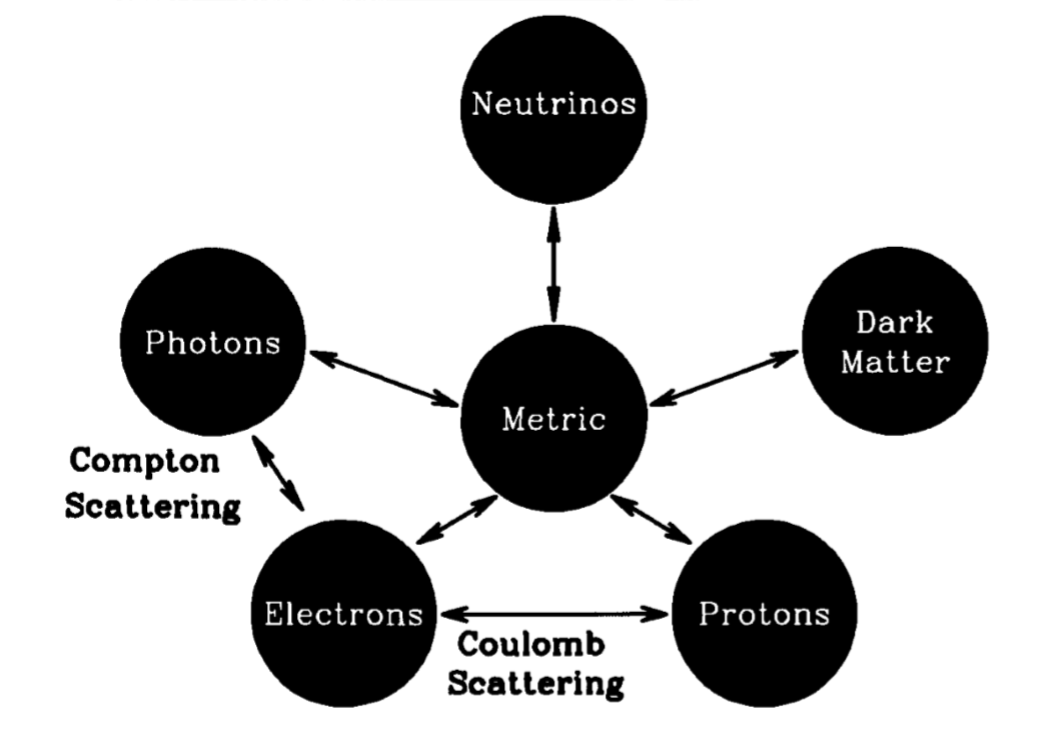
\includegraphics[width=\linewidth]{intm.png}
\end{figure}
\chapter{A critical overview of Cosmology}
Cosmology is an attempt to describe the universe as a whole and hence transcends the realms of all other branches of science. Any conclusion about the universe are bound to be profound and hence must be drawn with utmost caution. 

\chapter{The non linear Evolution}
\tbf{Q. Problem with linear peturbation theory:}
\begin{itemize}
\item It fails when the density contrast $\delta_k \approx 1$.
\end{itemize}
\tbf{Q. Why do we require a non linear evolution?}\\
\begin{itemize}
\item Most of the structures in the universe like galaxies, clusters have density contrast far less than 1. Hence, structurew can be best understood by a non linear theory.
\end{itemize}
\section{Spherical Model for the nonlinear collapse}
Our final verdict on the linear peturbation theory:
\begin{itemize}
\item From linear theory we where successfully able to arrive at the expression for processed power spectrum $P(k)$ at $t\geq t_{dec}$.
\item Our observation of the micro wave background radiation, guarantees that the density contrast had a value of $\delta_k \leq 10^{-4}$ or so at this epoch(this value of the density contrast is quite small).This small value implies that the peturbation can be studied as a linear theory and  this contrast evolves as $\propto \;\; a(t)$.
\item As the $\delta_k$ evolves as $\propto \;\; a(t) $, its value goes upto unity. Let this time be $t_{nl}$. Now this $t_{nl}$ is the time when non linear evolution kicks in and the linear peturbation theory fails for this particular mode of density contrast$\delta_k$.
\end{itemize} 
\tbf{Why where we using the fourier analysis in case of linear evolution of density?}\\

It is so because in linear evolution of $\delta(\mbf{x},t)$ under fourier transform, each mode $\delta_k(t)$ was evolving independently. Non this was true for linear evolution, and we don't have the same specific advantage from Fourier in nonlinear regime. Hence we will study the same in $\mbf{x}$ space as $\delta(\mbf{x},t)$.\\

\tbf{Q. Describe the formation of gravitationally bound system.}\\

\tit{Refer this to the paragraph 1 of Page 274 to Paddy's structure formation books.}\\
\medskip
While the simplest model for non linear evolution of density contrast is when we assume that the overdense region is a spherically symmetric one. Let us assume that the overdense region we are interested has an initial density distribution of 
\begin{equation}
\rho(r,t_i)=\rho_{b}(t_i)+\delta \rho(r,t_i)=\rho_b(t_i)\rr{1+\delta_i(r)}
\end{equation} 
Here $\delta_i(r)=\delta(r,t_i)$ is the initial density contrast which is some specified, non increasing function of $\tau$.\\

\tbf{Can we use Newtonian approximation to probe the evolution of such peturbation?}\\

Here we are interested in scales $\lambda<<d_H$, the size R of the overdense region can be takes to be very less than the hubble radius.\\
The dynamics of the overdense region is determined by the gravitational potential
\begin{equation*}
\Phi_{total}(r,t)=\Phi_{b}(r,t)+\delta \Phi_{b}(r,t)=-\frac{1}{2}\cc{\frac{\ddot{a}}{a}}r^2+\delta \Phi_{b}(r,t)
\end{equation*}
\begin{equation}
=\frac{2\pi}{3}G \rho_b r^2+\delta \Phi(r,t)
\end{equation} 
where $\Phi_b(r,t)$ is the equivalent newtonian potential of the friedman metric and $\delta \Phi$ is the potential generated due to the excess density.\\

The motion of a thin shell of particles located at a distance r is governed by the equation
\begin{equation}\label{eq:sppetur}
\frac{d^2 r}{d t^2}=-\nabla \Phi_{total}=-\frac{4 \pi G \rho_b(t)}{3}\mbf{r}-\nabla(\delta \Phi)=-\frac{GM_b}{r^3}\mbf{r}-\frac{G\delta M(r,t)}{r^3}\mbf{r}
\end{equation}
\begin{\cbox}
It is important to note that fir the spherically symmetric density distribution, the gravitational force only depend on the mass $\delta M$ contained inside the shell.
\end{\cbox} 
 Here, $M_b$ and $\delta M(r,t)$ stands for 
\begin{equation}
M_b=\frac{4\pi}{3}\rho_b(t)r^3=\frac{4\pi}{3}a^3(t)x^3=constant
\end{equation}
and
\begin{equation}
\delta M(r,t)=4\pi \int^r_0 \delta\rho(q,t)q^2dq=4 \pi \int^r_0 q^2 \delta (q,t) dq
\end{equation}
\begin{\cbox}
One more thing, to simplify our analysis, we assume that the spherical shell do not cross each other during the evolution. In such a case the mass contained within a shell of radius r does not change with time $\delta M(r,t)=\delta M(r_i,t_i)=$constant.
\end{\cbox}
 We can now combine the two terms in \eqref{eq:sppetur} and get
 \begin{equation}\label{eq:sppeturbmo}
 \frac{d^2 r}{dt^2}=-\frac{GM }{r^2}
 \end{equation}
 where,
 \begin{equation}
 M=M_b+\delta M=\rho_b\cc{\frac{4\pi}{3}r_i^3}(1+\bar{\delta_i})
 \end{equation}
 where
 \begin{equation*}
 \bar{\delta_i}=\cc{\frac{3}{4\pi r^3_i}}\int^{r_i}_0\delta_i(r) 4 \pi r^2
 \end{equation*}
 Here,
 \begin{itemize}
 \item $r_i$ is the initial radius of the mass M
 \item $\bar{\delta_i}$ is the average value of $\delta$ within $r_i$ at time $t_i$.
 
 \end{itemize}
 Integrating  \eqref{eq:sppeturbmo} we get
 \begin{equation}\label{eq:sppeturbsol}
 \frac{1}{2}\cc{\frac{dr}{dt}}^2-\frac{GM}{r}=E
 \end{equation}
 Here, E is the constant of integration.
 \begin{itemize}
 \item If $E>0$, $\frac{dr}{dt}>0$ and hence the shell is in an ever expanding phase.
 \item If $ E<0$, then as r increases, $\dot{r}$ will eventually become zero and later negative , implying a contraction and collapse.
 \end{itemize}
 In a more convenient form , let us express the equation \eqref{eq:sppeturbsol} at an initial time $t_i$.
 \begin{itemize}
 \item $t_i$ should be such that, $\delta$ is quite small such that we can claim that overdense region is expanding along with the background.
 \item or we can assume that peculiar velocities  are negligible at time $t=t_i$.
 \item $\dot{r}_i=\frac{\dot{a}}{a}r_i=H(t_i)r_i\equiv H_ir_i$ at time $t_i$
 \item the initial kinetic energy will be then defined as 
 \begin{equation}
 K_i\equiv\cc{\frac{\dot{r_i}^2}{2}}_{t=t_i}=\frac{H_i^2r_i}{2} 
 \end{equation}
\item  and the initial potential energy at $t=t_i$ is $U=-|U|$ and is defined as 
\begin{equation*}
|U|=\cc{\frac{GM}{r}}_{t=t_i}=\cc{\frac{G\rho_b\cc{\frac{4\pi}{3}r_i^3}(1+\bar{\delta_i})}{r_i}}=\cc{G\rho_b\cc{\frac{4\pi}{3}r_i^2}(1+\bar{\delta_i})}
\end{equation*} 
\begin{equation}
\implies |U|=\frac{1}{2}(1+\bar{\delta_i})H_i^2r_i^2=K_i\Omega_i(1+\bar{\delta_i})
\end{equation} 
Here, $\Omega_i=\cc{\frac{\rho_b(t_i)}{\rho_c(t_i)}}$ which denotes the initial value of the density parameter $\Omega$ of the smoothed background of universe.
\item And the total energy is given as 
\begin{equation}
E=K_i-K_i\Omega_i(1+\bar{\delta_i})=K_i\Omega_i[\Omega_i^{-1}-(1+\bar{\delta_i})]
\end{equation}
 \tbf{So, the condition $E<0$ for the shell to collapse (eventually), becomes $(1+\bar{\delta_i})>\Omega_i^{-1}$} or 
 \begin{equation}
 \bar{\delta_i}>[\Omega_i^{-1}-1]
 \end{equation}
  \item For a closed or a flat universe with $\cc{[\Omega_i^{-1}\leq 1]}$ this condition is satisfied . (Note even though overdesities will always collapse but the smaller overdensities will take more than the bigger overdensities to collapse.)For an open universe $\Omega_i<1$, the overdensity has to be above a critical radius to collapse such that $\bar{\delta_i}(r_{cr})=\Omega_i^{-1}$ to collapse.
\item 
 \end{itemize}
\section{N body simulation}
A universe constituted will collisionaless particles evolves only through gravity. This is how we study non linear evolution of density peturbations through N body simulation.\\

\tbf{Q. What does an N body simulation do?}\\
\begin{enumerate}
\item Here, the matter distribution is described as a collection of N particles interacting via gravity.
\item The state of the system at any time t is given by the position and velocity of the particles which are evolved through a sequence of small time steps.
\item The force on one particle by the rest N-1 particles is calculated when we have information of the particle position.
\item When we know force, we can update the particle positions again and go back to step 2.
\end{enumerate}
\tbf{Q. Is there any limitation to this stupendo-fantabulous method?}\\

Yes! the only limitation of the problem arises from the value of N which increases the time required for computation of forces.\\

After a brief introduction to N body simulation let us move to the next step that is the technique of the calculation.\\

Three different schemes have been popularly studied in the literature.
\begin{itemize}
\item P-P scheme (Particle Particle scheme)
\item The P-M scheme (Particle -Mesh scheme)
\end{itemize}
\subsection{The P-P method of N-body simulation}
This is the simplest of the algorithm where the force on each particle is calculated as a sum of inverse square law forces due to all other particles.\\

\begin{\cbox}
In general we don't calculate force all upto $\mbf{r}=0$, as the force $1/r^2$ blows up at zero; \tbf{what we do instead is smooth the law at small distances at small r and modifying }
\begin{equation}
\frac{1}{r^2}\rightarrow \frac{1}{r^2+a^2}
\end{equation}
\tit{although this smoothening would result in loss of spatial resolution, the computation becomes efficient.}
\end{\cbox}
\medskip
\tbf{Q. How does smoothening the scale makes calculation computationally efficient?}\\

Ans. As $r \rightarrow 0$ then, the velocities increase rapidly as $\frac{1}{r^2}\rightarrow \infty$. In order to keep track of such steep rise in velocities one has to use smaller time steps to follow the particle trajectory.\\

\tbf{Q. What are the disadvantages of PP scheme?}\\

Ans. In PP method, in order to calculate force on N particles due to (N-1) particles one has to do $N^2$
number of operations. Therefore, \tbf{PP scheme is employed for $N\leq 10^4$}.

\subsection{The PM scheme of N-body simulation}

Instead of making $N^2$ calculations through brute force by calculating force on each particle, one can instead \tbf{calculate force on each particle by first calculating potential (obtained from solving the Poisson equation on a mesh)}.
\subsubsection{Steps to apply PM algorithm}
\begin{itemize}
\item All the continuous variables in space e.g. density, potential are approximated by their values on a regular array of mesh points. \fn{ I think instead of the continuous function is space potential or density fields are approximated to a value for a given size of mesh and for the whole mesh one value is used for that variable. Therefore the implication being \tbf{the smaller the mesh the better?} }  .
\item Differential operators are replaced with finite difference approximations on the mesh.

\end{itemize}
 \chapter{MUSIC}
 
\end{document}
